% ══════════════════════════════════════════════════════════════════
% Fathom: The Cognitive Atlas
% Long-form arXiv synthesis (v1)
% Alexander Rodabaugh, Fathom Intelligence
% 2026-04-10
% ══════════════════════════════════════════════════════════════════

\documentclass[11pt,letterpaper]{article}
\usepackage{arxiv}
\usepackage[utf8]{inputenc}
\usepackage[T1]{fontenc}
\usepackage{lmodern}

\usepackage{tcolorbox}
\tcbuselibrary{skins,breakable}
\usepackage{enumitem}
\usepackage{siunitx}
\usepackage{xcolor}
\usepackage{etoolbox}
\usepackage{microtype}
\usepackage{seqsplit}
% Allow line breaks inside long typewriter paths / filenames with underscores
\newcommand{\pbs}[1]{\texttt{\seqsplit{#1}}}
% Slightly more tolerant line breaking for a 29-page long-form paper
\tolerance=1500
\emergencystretch=3em
\hbadness=2000

\definecolor{fathomblue}{RGB}{30,55,110}
\definecolor{fathomred}{RGB}{176,30,46}
\definecolor{fathomgreen}{RGB}{10,138,79}
\definecolor{fathomamber}{RGB}{194,131,0}
\definecolor{fathomlight}{RGB}{234,238,246}
\definecolor{fathomgrey}{RGB}{85,85,85}

\graphicspath{{./}{../}{figures/}{../figures/}}

% Reproducibility anchor symbol (inline)
\newcommand{\repro}[1]{%
  \textcolor{fathomgreen}{\footnotesize$\bigstar$\,\texttt{#1}}}

% Measurement card environment
\newtcolorbox{mcard}[2][]{%
  enhanced,
  colback=fathomlight,
  colframe=fathomblue,
  boxrule=0.8pt,
  arc=3pt,
  left=8pt, right=8pt, top=6pt, bottom=6pt,
  title={\textcolor{white}{\bfseries #2}},
  fonttitle=\normalsize,
  coltitle=white,
  #1
}

% Executive summary environment
\newtcolorbox{execbox}{%
  enhanced,
  colback=white,
  colframe=fathomblue,
  boxrule=1.2pt,
  arc=4pt,
  left=12pt, right=12pt, top=10pt, bottom=10pt,
  title={\textcolor{white}{\bfseries EXECUTIVE SUMMARY}},
  fonttitle=\large,
  coltitle=white,
  breakable,
}

\title{\textcolor{fathomblue}{The Fathom Cognitive Atlas}\\[4pt]
       \large Cross-Architecture Measurement Science for Transformer Internals}
\author{Alexander Rodabaugh\\
        Fathom Intelligence\\
        \texttt{heyzoos123@gmail.com}}
\date{April 10, 2026}

\begin{document}
\maketitle

% ══════════════════════════════════════════════════════════════════
% EXECUTIVE SUMMARY (page 1)
% ══════════════════════════════════════════════════════════════════
\begin{execbox}

\textbf{Problem.} Mechanistic interpretability findings do not transfer across
architectures. SAE features trained on Gemma say nothing about Llama; a
jailbreak circuit identified in Qwen may or may not exist in Phi. Every result
is one-model-local because every method is one-model-local.

\textbf{Contribution.} We present \textsc{Fathom}, a suite of five cognitive
measurement instruments for transformer internals, culminating in an
\emph{architecturally universal} primitive
$D \;=\; \cos\!\big(\mathbf{h}^{(L)},\;\mathbf{w}_{y_t}\big)$ that is computable
on any transformer from the final-layer residual stream and the unembedding
row of the chosen token, without SAE, per-model probes, or architecture-specific
infrastructure.

\textbf{Validation.} We run the first \emph{pre-registered cross-architecture
replication} of an RLHF convergence effect. Six model families (Gemma-2-2B,
Llama-3.2-3B, Qwen2.5-3B, Gemma-3-1B, Llama-3.2-1B, Qwen2.5-1.5B), each in
base and instruct form, captured on a fixed 90-prompt probe set.
Pre-registration \textsc{sealed} in git commit \texttt{e32cc75}
\textbf{93 minutes before any v0.3 data was captured}; the decision rule was
applied without modification after data collection.

\vspace{4pt}
\begin{center}
\begin{tabular}{lll}
\toprule
\textbf{Sealed condition} & \textbf{Threshold} & \textbf{Observed} \\
\midrule
Mean entropy-early LOO cosine & $\geq\, 0.40$ & \textcolor{fathomgreen}{$\mathbf{+0.769}$} \\
Permutation $p$ (one-sided, $n\!=\!2000$) & $<\, 0.05$ & \textcolor{fathomgreen}{$\mathbf{0.0315}$} \\
Bootstrap 95\% CI on mean & lower $>\, 0$ & \textcolor{fathomgreen}{$\mathbf{[+0.571,\,+0.869]}$} \\
\midrule
\textbf{Verdict} & & \textbf{\textcolor{fathomgreen}{H1 SUPPORTED}} \\
\bottomrule
\end{tabular}
\end{center}
\vspace{4pt}

\textbf{All 6 of 6} families show positive leave-one-out cosines.

\textbf{Public artifacts.}
\textbullet\; Paper v15 \textit{(unified release: paper + atlas data
bundle as sibling files on one Zenodo record)}:
\texttt{doi.org/10.5281/zenodo.19504993}
(concept \texttt{10.5281/zenodo.19326174})\\
\textbullet\; OSF mirror: \texttt{osf.io/wtkzg/}\\
\textbullet\; Reproducibility script: \texttt{verify\_all\_claims.py}
(28 assertions, runs under 1 minute on CPU)

\textbf{This paper is NOT.}
\textbullet\; A claim that we have solved alignment, oversight, or
interpretability.
\textbullet\; A claim that RLHF is universally convergent across all
architectures: $n\!=\!6$ includes three scale/generation variants and is
weaker than $n\!=\!6$ with truly independent families would have been. This
limitation is stated in \S\ref{sec:limitations}.

\end{execbox}

% ══════════════════════════════════════════════════════════════════
% ABSTRACT
% ══════════════════════════════════════════════════════════════════
\begin{abstract}
Mechanistic interpretability findings do not transfer across architectures,
and published results are almost never pre-registered. We show that both
can change at once. We identify an architecturally universal measurement
primitive, $D\,=\,\cos(\mathbf{h}^{(L)},\mathbf{w}_{y_t})$ --- the cosine
between the final-layer residual stream and the unembedding row of the
chosen token --- which requires no SAE, no per-model training, and is
well-defined on any transformer with an explicit unembedding. A
preliminary orthogonality check at $n\!=\!5$ places $D$ inside the
cognitive-geometry family as an SAE-free approximation to late-layer
commitment geometry ($r\,\approx\,0.99$ with the SAE-derived $C_\Delta$),
not as a new independent axis. We then use $D$ and a validated entropy
proxy to run a pre-registered cross-architecture replication of an RLHF
convergence effect on twelve open-weight captures (six families
$\times$ base/instruct), sealed in git commit \texttt{e32cc75} ninety-three
minutes before any of the new data was captured. The sealed decision rule
declared three conditions for the primary measurement; they were applied
without modification after the data landed. All three passed: mean
leave-one-out cosine $+0.769$ (threshold $\geq 0.40$), permutation
$p\,=\,0.0315$ (threshold $<\,0.05$), bootstrap 95\% confidence interval
$[+0.571,\,+0.869]$ (threshold lower bound $>\,0$). All six of six
families show positive leave-one-out cosines. \textbf{H1 is supported.}
We release the complete Fathom Cognitive Atlas v0.3 --- probe set, twelve
open-model captures plus one closed-model exploratory capture via logprob
API, full analysis code, bulletproof audit, and sealed pre-registration
--- as sibling files on a single Zenodo record (paper v15,
\texttt{10.5281/zenodo.19504993}) under the Fathom concept DOI
\texttt{10.5281/zenodo.19326174}, with CC-BY-4.0 on the data and MIT
on the code. The primary contribution is methodological: pre-registered
statistical rigor, architectural universality, and public reproducibility
can coexist in a single interpretability paper. The empirical result
(RLHF convergence replicating at $n\!=\!6$ families including three
scale/generation variants) is the demonstration payload, with the
within-family-variance caveat stated explicitly in
\S\ref{sec:limitations}. Three of the secondary Fathom instruments ---
the SAE-based commitment intensity $S$, the coherence spectrum Gini
metric, and the cognitive autopsy layer-11 localization on Gemma-2-2B ---
are supporting material and are detailed in the appendices. We also
include a post-pilot exploratory finding and its pre-registered
sensitivity test (\S\ref{sec:spectral}): Fourier analysis of the
$C_\Delta(t)$ coherence trajectory shows a bin-localized directional
pattern (correct generations carrying more spectral power than
hallucinated ones at a model-specific peak period) that replicates
across architectures and across Fathom's v21 and v22 labelings but
does not survive a pre-registered family-wise $p\,<\,0.05$ threshold
across $20$ frequency bins at current sample sizes. The peak bin and
the direction replicate robustly; the family-wise correction fails.
We report this outcome honestly against the sealed decision rule and
propose a bin-locked confirmatory design as the immediate next step.
The frequency-domain framing is inspired by \citet{weng2026sustained}
and constitutes the first link from Fathom to the frequency-domain
tradition in cognitive neuroscience.
\end{abstract}

% ══════════════════════════════════════════════════════════════════
% 1. INTRODUCTION
% ══════════════════════════════════════════════════════════════════
\section{Introduction}
\label{sec:intro}

Mechanistic interpretability has a portability problem. A hallucination
circuit identified in Gemma-2-2B may or may not exist in Llama-3.2-3B. A
sparse autoencoder trained on Mistral will tell you nothing about Phi until
you train another. A jailbreak vulnerability observed in Qwen does not
predict the same vulnerability in an unrelated architecture. Every positive
result is one-model-local because every method is one-model-local: SAEs are
trained per architecture, probes are fit per task, activation patching is
done per checkpoint. Knowledge compounds slowly because nothing generalizes
automatically.

Meanwhile, the frontier of alignment is raising the stakes. \citet{song2026peer}
show that frontier models spontaneously develop peer-preservation behaviors,
deceiving oversight systems to protect allied models --- an emergent
collusion that makes semantic-level monitoring unreliable. \citet{anthropic2026emotion}
demonstrate causal internal emotion representations in language models,
validating the premise that internal state carries information the output
does not. Both findings point the same direction: oversight must move below
the semantic layer, into the geometry of the computation itself. But moving
below the semantic layer inherits the portability problem: you cannot audit
a fleet of heterogeneous models with a probe that only works on one of them.

\paragraph{The measurement-science alternative.} We propose that the field
needs cognitive \emph{measurement instruments} rather than more cognitive
\emph{explanations}: architecturally universal primitives that produce
comparable numbers across models, with pre-registered statistical rigor, and
with public reproducibility kits that let anyone independently verify the
numbers. This is how thermodynamics progressed (thermometers before steam
engines) and how neuroscience progressed (electrodes before circuits). We
apply the same pattern to transformer internals.

\paragraph{The Fathom suite.} This paper presents five such instruments:
computational depth $K$ (prior work), per-layer coherence $C$ and its
late-minus-early delta $C_\Delta$, the commitment intensity $S$ grounded in
the inverse participation ratio of condensed-matter physics, and the
architecturally universal honesty axis
$D\,=\,\cos(\mathbf{h}^{(L)},\mathbf{w}_{y_t})$. The $D$ axis is the key
contribution for cross-architecture work: it reduces to a single per-token
dot product between the final-layer residual stream and the unembedding row
of the chosen token, requires no SAE, and is well-defined for any
transformer with an explicit unembedding. The other four instruments require
SAE decomposition and are therefore currently limited to models with public
SAEs (Gemma, Llama for the experiments reported here), but we show that the
entropy proxy of the logit distribution reproduces the $D$-axis signal
sufficiently well to extend Fathom measurements to any model with an
API-exposed logprob interface, bridging to the closed-weight frontier.

\paragraph{The cross-architecture replication.} We use the suite to run a
\emph{pre-registered cross-architecture replication of an RLHF
convergence effect}. Six model families, each in base and instruct form,
processed on a fixed 90-prompt probe set. The hypothesis (the ``RLHF
Attractor'' of \S\ref{sec:atlas}): instruct models from different
architectures move in a consistent direction relative to their own base
models in cognitive signature space, such that an attractor centroid
computed from other families' instruct-minus-base deltas predicts any held-
out family's own instruct-minus-base delta with positive leave-one-out
cosine. The pre-registration was sealed in git before any v0.3 data was
captured; the three-condition decision rule was applied without
modification; all three conditions passed at $n\!=\!6$.

\paragraph{Contributions.}
\begin{enumerate}[leftmargin=18pt,itemsep=2pt,topsep=3pt]
\item We formalize the \emph{Fathom measurement instrument suite}: five
cognitive axes with explicit architectural requirements, orthogonality
analysis, and source JSONs for every numerical claim.
\item We derive the commitment intensity measurement from the inverse
participation ratio and verify the equivalence to machine precision on real
trajectories, grounding the instrument in a seventy-year theoretical
lineage.
\item We run a pre-registered cross-architecture replication of an
RLHF convergence effect at $n\!=\!6$ families, sealed in git 93 minutes
before data capture, and show \textbf{H1 supported} on all three decision
conditions (\S\ref{sec:atlas}). To our knowledge, this is the first such
pre-registered interpretability replication; we discuss comparison to
prior work in \S\ref{sec:discussion}.
\item We release the \emph{Fathom Cognitive Atlas v0.3}: probe set, twelve
open-model captures plus one closed-model capture, six findings documents,
sealed pre-registration, bulletproof audit, and a reproducibility script
with 28 assertions, under CC-BY-4.0 / MIT, with its own Zenodo concept DOI
(\texttt{10.5281/zenodo.19502715}).
\end{enumerate}

\paragraph{What is new in this paper relative to prior Fathom releases.}
The Fathom project has evolved publicly through fourteen Zenodo versions
(concept DOI \texttt{10.5281/zenodo.19326174}). The material on
computational depth $K$, per-layer coherence $C$, the coherence delta
$C_\Delta$, the commitment intensity $S$ and its IPR grounding, the
coherence spectrum with the Gini AUC result, the cognitive autopsy at
layer 11, and the $D$-axis jailbreak pilot all pre-date this paper and
are published as Fathom paper v14
(\texttt{10.5281/zenodo.19502710}). This arXiv submission contributes three
pieces not present in any prior version: (i)~the sealed pre-registration
of an RLHF cross-architecture convergence hypothesis (committed as
\texttt{e32cc75} ninety-three minutes before any v0.3 capture);
(ii)~the Cognitive Atlas v0.3 pre-registered replication at $n\!=\!6$
families with all three sealed conditions passing
(\S\ref{sec:atlas}; released separately as
\texttt{10.5281/zenodo.19502716}); and (iii)~the bulletproof audit that
withdrew the earlier v0.2.1 ``Qwen anomaly'' framing after bootstrap and
permutation analysis showed it was noise at $n\!=\!3$ (detailed in
\S\ref{sec:atlas}). The previously published material on $K$, $C$,
$C_\Delta$, $S$, IPR, and the coherence spectrum is briefly summarised in
\S\ref{sec:instruments}--\ref{sec:supporting} and given in full in
Appendices~\ref{app:diagnosis} and \ref{app:validation}, so that this
paper is self-contained.

\paragraph{Paper roadmap.} Section~\ref{sec:related} places this work
against existing SAE, behavioural detector, representation engineering,
and contrastive decoding literatures. Section~\ref{sec:instruments}
defines the five measurement instruments as a suite of cards.
Section~\ref{sec:ipr} develops the IPR physics grounding of $S$.
Section~\ref{sec:supporting} summarises the single-model supporting
evidence (full detail in Appendices~\ref{app:diagnosis}
and~\ref{app:validation}). Section~\ref{sec:atlas} is the centrepiece:
the cross-architecture pre-registered replication.
Section~\ref{sec:falsify} states what would have falsified H1.
Section~\ref{sec:limitations} is honest about null results and scope
corrections, with particular attention to the $n\!=\!6$ scale-variant
caveat in \S\ref{sec:lim-n6}. Section~\ref{sec:predictions} states
broader theoretical predictions that others can test.
Section~\ref{sec:discussion} is the discussion. Appendices contain
per-family numerics, git chronology, deviations from pre-registration,
the IPR derivation in full, and the single-model evidence in full.

% ══════════════════════════════════════════════════════════════════
% 2. RELATED WORK
% ══════════════════════════════════════════════════════════════════
\section{Background and related work}
\label{sec:related}

\paragraph{Sparse autoencoder feature interpretation.} SAEs decompose
transformer residual streams into interpretable monosemantic features
\citep{cunningham2023sparse, bricken2023monosemanticity, templeton2024scaling}.
This line of work operates under the paradigm of \emph{finding the feature
that explains behaviour X} --- a causal interpretability program. Our work
extends SAEs in a different direction: from interpretability tool to
\emph{measurement infrastructure}. We show that SAE decomposition enables
the extraction of quantitative cognitive properties (coherence geometry)
that are inaccessible to raw activation analysis, and that those properties
in turn admit an architecturally universal approximation via the $D$-axis.

\paragraph{Behavioural hallucination detection.} Semantic entropy
\citep{farquhar2024semantic} requires multiple samples and operates on
output-level representations. SelfCheckGPT \citep{manakul2023selfcheckgpt}
operates on outputs. DoLa \citep{chuang2024dola} contrasts layer
predictions to modify decoding but does not measure internal state.
Semantic uncertainty \citep{kuhn2023semantic} generalizes
entropy to semantic clusters. None of these methods measure per-token
SAE-derived commitment geometry, and none of them have demonstrated
head-to-head superiority with pre-registered decision rules on open-weight
models. Our $S_{\text{early}}$ instrument beats logit entropy head-to-head
(AUC $0.663$ vs. $0.607$, $p\,=\,0.013$) on the same 200 TruthfulQA items.

\paragraph{Representation engineering and inference-time intervention.}
Representation Engineering \citep{zou2023representation} identifies
high-level concept directions in activation space and manipulates them to
steer behavior. Inference-Time Intervention \citep{li2024iti} finds
``truthful'' attention heads and boosts them at inference. Both operate on
representations, both produce steering interventions, but neither formalizes
a measurement instrument with pre-registered statistical rigor across
architectures. Our contribution is complementary: we measure, they steer.

\paragraph{Inverse participation ratio.} The IPR measures localization in
discrete distributions \citep{anderson1958absence}. High IPR means localized
(a few sites carry all the weight); low IPR means delocalized (weight is
spread evenly). The IPR has been used in quantum many-body physics, random
matrix theory, and disordered systems for more than seventy years. It is
a mature theoretical construct. We show that the Fathom commitment intensity
$S$ \emph{is} a specific IPR applied to coherence event trajectories. This
is not a post-hoc interpretation; it is a derivation.

\paragraph{Biological parallel: sustained alpha oscillations as
attentional prioritization.}
Recent work in human cognitive neuroscience provides a striking biological
analog to $S_{\text{early}}$ as a commitment-intensity instrument.
\citet{weng2026sustained} use EEG in a two-item working-memory paradigm
with prioritized and deprioritized items across short ($1$ s) and long
($3$ s) delays. They report that sustained alpha-band power tracks the
\emph{prioritized} item throughout the delay with reliable decodability,
while the deprioritized item transitions to an activity-quiescent state
with no sustained alpha signature --- a dissociation between
prioritization and maintenance. The underlying measurement is
time-localization: how concentrated the alpha envelope remains on a
single representational target across a delay window. Our
$S_{\text{early}}$ instrument measures an analogous cognitive property in
transformer residual streams: a token-localization measure (via IPR on
coherence event trajectories) of how concentrated the model's commitment
remains on a single attractor across the early generation window. Both
measure \emph{which cognitive target the system is actively prioritizing
right now}, and both distinguish prioritization from mere storage
--- $S_{\text{early}}$ is orthogonal to $K$ (computational depth) in
Fathom, just as sustained alpha is dissociated from contralateral delay
activity in working memory \citep{weng2026sustained}. We flag this
parallel explicitly: we make no causal claim of identity, but the
substrate-independent ``localization of active selection'' construct
that both measurements target is, in our view, the most promising
direction for cross-substrate validation of $S$ as a measurement
instrument rather than an architecture-specific heuristic.

\paragraph{The measurement-science gap.} The above literatures collectively
operate on three paradigms: \emph{find the feature} (SAE circuits),
\emph{detect the output} (behavioral detectors), \emph{steer the computation}
(representation engineering). None of them constitute a measurement-science
paradigm, by which we mean: (i) architecturally universal primitives,
(ii) pre-registered statistical rigor, (iii) public reproducibility kits
that let anyone verify the numbers without access to the original lab.
Fathom targets that gap.

% ══════════════════════════════════════════════════════════════════
% 3. MEASUREMENT INSTRUMENTS
% ══════════════════════════════════════════════════════════════════
\section{The Fathom measurement instrument suite}
\label{sec:instruments}

This section presents the five cognitive measurement instruments as a
standardized suite of \emph{measurement cards}. Each card gives the formal
definition, the architectural requirements, the cross-architecture validation
status, the effect size of the primary validation study, and the source
JSON file containing the underlying numerical data. The cards are designed
to be scannable: a reviewer should be able to compare the instruments at a
glance without reading the full method section.

\subsection{K --- Computational Depth}

\begin{mcard}{K --- Computational Depth (prior work)}
\textbf{Definition.} $K$ is the attribution-weighted mean layer index of
the SAE features active in predicting the next token. Higher $K$ means
computation concentrated in later layers; lower $K$ means earlier layers.
\vspace{2pt}

\textbf{Requirements.} Full SAE decomposition across all layers. Circuit
tracer or equivalent attribution pipeline.
\vspace{2pt}

\textbf{Cross-architecture status.} Originally reported on Gemma-2-2B.
Cross-architecture value as a stand-alone hallucination detector is
\emph{limited}: $K$ was at chance on TruthfulQA ($d\,=\,+0.11$,
AUC $\,=\,0.55$) in the spectrum analysis of Appendix~\ref{app:diagnosis}. It remains
useful as a descriptor of where computation happens, not as a discriminator
of what kind of computation happens.
\vspace{2pt}

\textbf{Validation.} Published in Fathom v2 (\texttt{10.5281/zenodo.19327451})
with $p\,=\,0.000051$, $d\,=\,0.5$ on surface-recall vs. explanatory-reasoning
contrasts, $n\!=\!30$ pairs, Gemma-2-2B.
\vspace{2pt}

\textbf{Source.} \repro{paper/figures/fig1\_depth\_scale.pdf} (prior
Fathom v2 figure, referenced for historical context, not reused in this
paper's results).
\end{mcard}

\subsection{C and $C_\Delta$ --- Per-layer coherence and its delta}

\begin{mcard}{C --- Per-layer Coherence}
\textbf{Definition.} For each generated token $t$, the per-layer coherence
$C_\ell(t)$ is the mean pairwise cosine similarity of the top-$k$ SAE
transcoder decoder directions active at layer $\ell$:
\[
C_\ell(t) \;=\; \frac{1}{\binom{k}{2}} \sum_{i<j}
\frac{\mathbf{d}_i\cdot\mathbf{d}_j}{\|\mathbf{d}_i\|\|\mathbf{d}_j\|}
\]
\vspace{-8pt}

\textbf{Requirements.} SAE transcoder (not encoder) access with decoder
vectors. Circuit tracer \texttt{TranscoderSet} or equivalent.
\vspace{2pt}

\textbf{Cross-architecture status.} SAE-limited. Currently reported on
Gemma-2-2B base and instruct.
\vspace{2pt}

\textbf{Source.} \repro{truthfulqa\_results/S\_truthfulqa\_n200.json}.
\end{mcard}

\begin{mcard}{$C_\Delta$ --- Coherence Delta (late $-$ early)}
\textbf{Definition.} $C_\Delta(t) \,=\, \bar{C}_{\text{late}}(t) \,-\,
\bar{C}_{\text{early}}(t)$, where early means the first third of network
layers and late means the last third. Positive $C_\Delta$ means the model's
late-layer features are more self-coherent than its early-layer features
at that token --- a signature of late-layer concept lock-in.
\vspace{2pt}

\textbf{Requirements.} Per-layer $C$ coverage. SAE-limited.
\vspace{2pt}

\textbf{Cross-architecture status.} SAE-limited. Validated as a
hallucination signature on Gemma-2-2B: TruthfulQA $n\!=\!50$ pilot,
$p\,=\,0.040$, $d\,=\,0.407$, AUC $\,=\,0.582$ for hallucinated over
correct. This is the ``wrong attractor'' signature.
\vspace{2pt}

\textbf{Source.}
\repro{truthfulqa\_results/cognitive\_divergence\_analysis.json}.
\end{mcard}

\subsection{S --- Commitment intensity}

\begin{mcard}{S --- Commitment Intensity (IPR)}
\textbf{Definition.} $S$ is the ratio of the maximum coherence delta to the
number of supra-threshold events:
\[
S \;=\; \frac{\max_t\,C_\Delta(t)}{|\{t : C_\Delta(t)>\tau\}|}
\qquad (\tau\,=\,0.005,\;\text{fixed})
\]
Mathematically equivalent to $S\,=\,M\cdot\text{IPR}(\hat{e})$ with
$M\,=\,\max_t C_\Delta(t)$ and $\text{IPR}(\hat{e})\,=\,1/K_\tau$ the
inverse participation ratio of the uniform event-location distribution
(see \S\ref{sec:ipr}).
\vspace{2pt}

\textbf{Requirements.} Per-token $C_\Delta$ trajectory. SAE-limited for the
exact ratio form; the entropy proxy of \S\ref{sec:atlas} reproduces enough
of the signal to extend to SAE-free models.
\vspace{2pt}

\textbf{Cross-architecture status.} Validated on two architecture families
(Gemma-2-2B, Llama-3.2-1B-Instruct) with architecture-adaptive windows.
Fisher combined $p\,=\,0.0006$.
\vspace{2pt}

\textbf{Effect size.} Cross-dataset meta-analysis across three independent
designs (Gemma-2-2B base hedge/commit paired $n\!=\!30$, Gemma-2-2B-IT
hedge/commit paired $n\!=\!30$, TruthfulQA unpaired $n\!=\!94$), pooled
$d\,=\,+0.494$, Fisher combined $p\,=\,0.0008$. Subsample robustness:
95.8\% of 50\%-subsamples show $d\,>\,0$ across all three datasets.
\vspace{2pt}

\textbf{Source.}\\
\repro{truthfulqa\_results/baselines\_headtohead.json}\\
\repro{truthfulqa\_results/S\_baselines\_n200.json}
\end{mcard}

\subsection{D --- Honesty axis (architecturally universal)}

\begin{mcard}{D --- Honesty Axis (SAE-free)}
\textbf{Definition.} For generation step $t$ with final-layer residual
$\mathbf{h}_t^{(L)}$ and chosen token $y_t$ with unembedding row
$\mathbf{w}_{y_t}$:
\[
D_t \;=\; \frac{\mathbf{h}_t^{(L)}\cdot\mathbf{w}_{y_t}}
                {\|\mathbf{h}_t^{(L)}\|\,\|\mathbf{w}_{y_t}\|}
\;\in\;[-1,+1]
\]
High $D$: the residual points at the emitted token (the computation
supports the expression). Low $D$: the residual points elsewhere.
\vspace{2pt}

\textbf{Requirements.} Final-layer residual stream and the unembedding
matrix. \emph{No SAE}. \emph{No per-model training}. Both exist by
construction on every transformer with an explicit unembedding, so $D$ is
architecturally universal.
\vspace{2pt}

\textbf{Cross-architecture status.} Validated on six models from three
families (Gemma-2-2B, Llama-3.2-3B, Qwen2.5-3B, each $\pm$ RLHF), each on
$n\!=\!30$ matched direct/adversarial prompt pairs. Fisher combined $p
\,<\,10^{-14}$. Pre-registered on OSF (\texttt{osf\_prereg\_d\_axis.md})
before any data was collected.
\vspace{2pt}

\textbf{Scope correction.} A preliminary $n\!=\!5$ orthogonality check
found $D$ correlates strongly with $C_\Delta$ on paired deltas
($r\,\approx\,+0.99$). We therefore reframe $D$ as an \emph{SAE-free proxy
for late-layer commitment geometry}, not as an independent fifth cognitive
axis. This is the key limitation of the fifth instrument; the scope
correction is retained in \S\ref{sec:limitations}.
\vspace{2pt}

\textbf{Strongest single signal.} Qwen2.5-3B base, $d_z\,=\,-1.86$
(paired), $p\,=\,4.6\!\times\!10^{-11}$ for the direct vs. adversarial
contrast.
\vspace{2pt}

\textbf{Source.} \repro{figures/d\_axis\_cross\_arch.png},
\repro{atlas/captures/*.json} (all 12 open-model captures).
\end{mcard}

\subsection{Orthogonality of the suite}
\label{sec:orthogonality}

On $n\,=\,400$ pooled TruthfulQA samples (200 correct + 200 hallucinated,
Gemma-2-2B), the four SAE-based axes are mutually independent:
$|r|<0.10$ for every pair of $\{K,C,C_\Delta,S\}$
(Table~\ref{tab:orth} and Figure~\ref{fig:fourax}).

\begin{table}[h]
\centering
\small
\begin{tabular}{lcccc}
\toprule
 & $K$ & $C$ & $C_\Delta$ & $S$ \\
\midrule
$K$       & $1.00$  & $-0.02$ & $-0.10$  & $-0.06$ \\
$C$       &         & $1.00$  & $+0.02$  & $+0.03$ \\
$C_\Delta$&         &         & $1.00$   & $-0.003$ \\
$S$       &         &         &          & $1.00$ \\
\bottomrule
\end{tabular}
\caption{Pairwise Pearson correlations among the four SAE-based cognitive
axes on $n\!=\!400$ pooled TruthfulQA samples (Gemma-2-2B). All off-diagonal
$|r|\!<\!0.10$, confirming mutual independence.
\repro{truthfulqa\_results/S\_baselines\_n200.json}}
\label{tab:orth}
\end{table}

\begin{figure}[h]
\centering
\includegraphics[width=0.55\linewidth]{fig2_four_axis_correlation.png}
\caption{Five-axis correlation matrix for the Fathom suite. The four
SAE-based axes ($K$, $C$, $C_\Delta$, $S$) are mutually independent at
$|r|\!<\!0.10$. The fifth axis $D$ correlates at $r\!\approx\!+0.99$ with
$C_\Delta$ on paired deltas from a $n\!=\!5$ pilot, which is why we
reframe $D$ as an SAE-free proxy rather than an independent fifth axis.
The $D$-to-$\{K,C,S\}$ correlations are not yet measured; those cells are
shown as dashes.}
\label{fig:fourax}
\end{figure}

% ══════════════════════════════════════════════════════════════════
% 4. IPR PHYSICS GROUNDING
% ══════════════════════════════════════════════════════════════════
\section{Physics grounding: S as inverse participation ratio}
\label{sec:ipr}

The commitment intensity $S$ is not an ad hoc formula. It is mathematically
exactly the inverse participation ratio (IPR) of the coherence event
distribution, a seventy-year-old construct from condensed-matter physics
and random matrix theory \citep{anderson1958absence}.

\paragraph{The IPR construct.} Given a non-negative distribution
$\hat{e}\,=\,(e_1,\dots,e_n)$ over $n$ sites with $\sum_i e_i\,=\,1$, the
participation ratio is $\text{PR}(\hat{e})\,=\,1/\sum_i e_i^2$. It measures
effective support size: if all mass is on one site, PR $=1$; if mass is
uniform, PR $\,=\,n$. The inverse participation ratio
$\text{IPR}\,=\,\sum_i e_i^2\,=\,1/\text{PR}$ measures localization: high
IPR means localized (a few sites carry all the weight); low IPR means
delocalized. The IPR appears in Anderson localization, Edwards--Thouless
theory, random matrix eigenvector statistics, quantum many-body physics,
and discrete distribution analysis broadly.

\paragraph{Fathom derivation.} Define the coherence event distribution by
identifying every token position $t$ whose $C_\Delta(t)>\tau$ as a ``site''
with unit weight, and normalizing by the number of events $K_\tau$. The
distribution is uniform over the active positions. Its IPR on this uniform
distribution over $K_\tau$ sites is exactly $1/K_\tau$. Multiplying by the
peak magnitude $M\,=\,\max_t C_\Delta(t)$ gives $S\,=\,M\cdot(1/K_\tau)\,=\,
\max_t C_\Delta(t)\,/\,K_\tau$, which is identical to the Fathom definition.
The equivalence holds exactly and has been verified to machine precision
on ten real TruthfulQA trajectories.

\paragraph{Why the ratio form is specific.} The cross-dataset meta-analysis
of Appendix~\ref{app:validation} tested three candidate metrics across the three
independent datasets: the ratio $S\,=\,M/K_\tau$, the max alone $M$, and
the mean of $C_\Delta$ over the trajectory. Only the ratio form replicates
in all three datasets (pooled $d\,=\,+0.498$). The max alone fails
(pooled $d\,=\,+0.309$, inconsistent direction across datasets) and the
mean alone fails (pooled $d\,=\,+0.067$, no signal). The IPR framing
explains why: max alone captures peak magnitude but not event sparsity;
mean alone captures neither. Only the ratio captures both, which is
exactly what the IPR prescribes. This is metric-specificity in the
measurement-theory sense: a single specific functional form is required,
and the form comes out of physics, not post-hoc tuning.

\begin{figure}[h]
\centering
\includegraphics[width=0.9\linewidth]{figA_ipr_physics.png}
\caption{Left: localized vs. delocalized event distributions over token
positions. Localized (high $S$): few intense commitment events. Delocalized
(low $S$): many distributed small events. Right: the $S\,=\,M\cdot
\text{IPR}(\hat{e})$ equivalence and a numerical example on synthetic
distributions showing a ratio separation of about $5\times$, matching the
cross-dataset $d\,\approx\,0.5$ we observe empirically.}
\label{fig:ipr}
\end{figure}

% ══════════════════════════════════════════════════════════════════
% 5. SINGLE-MODEL SUPPORTING EVIDENCE (brief summary)
% Full details in Appendices B (diagnosis) and C (validation)
% ══════════════════════════════════════════════════════════════════
\section{Single-model supporting evidence}
\label{sec:supporting}

Before presenting the cross-architecture replication that is the
centrepiece of this paper, we briefly summarise the single-model
supporting evidence that motivates the measurement approach. Full tables,
figures, and methodology for this section are in
Appendices~\ref{app:diagnosis}~and~\ref{app:validation}.

\paragraph{Mechanistic diagnosis (Gemma-2-2B only; see
Appendix~\ref{app:diagnosis}).} The \emph{shape} of the per-layer
coherence distribution carries discriminative information that scalar
summaries discard. On $n\,=\,200$ TruthfulQA correct/hallucinated items,
the Gini coefficient of the per-layer coherence spectrum achieves
AUC\,$=\,0.685$, while scalar $K$ (depth) is at chance (AUC\,$=\,0.550$).
Thirteen of sixteen spectrum metrics survive Holm--Bonferroni correction.
A per-layer cognitive autopsy localizes the hallucination signal at
layer~11 ($p\,=\,2.7\!\times\!10^{-12}$, primary fault locus in 63\% of
hallucinations) with layers 11--12 jointly carrying 41\% of all excess
coherence. This identifies hallucination as a coherence
\emph{concentration} phenomenon, not a shift in computational depth ---
a finding that is specific to the tested model and that we do not claim
generalises across architectures without further replication.

\paragraph{Single-instrument validation
(see Appendix~\ref{app:validation}).} The SAE-based commitment intensity
$S_{\text{early}}$ (first seven tokens) replicates with consistent effect
size across three independent experimental designs: Gemma-2-2B base
hedge/commit ($d\,=\,+0.501$, $n\,=\,30$ paired), Gemma-2-2B-IT
hedge/commit ($d\,=\,+0.466$, $n\,=\,30$ paired), and Gemma-2-2B-IT
TruthfulQA ($d\,=\,+0.506$, $n\,=\,94$ unpaired). Pooled meta-effect is
$d\,=\,+0.494$, Fisher combined $p\,=\,0.0008$ (one-sided). $S_{\text{early}}$
beats logit entropy in a head-to-head on the same 200 TruthfulQA items
(AUC\,$=\,0.663$ vs.\ $0.607$, $p\,=\,0.013$). Three SAE-free probes on
four architecture families all fail (Fisher combined $p\,>\,0.6$ each),
establishing that the SAE decomposition is performing measurement work
that raw activation analysis cannot.

\paragraph{What role these play in the paper.} The supporting evidence
above establishes that (i)~per-layer coherence geometry is a real
discriminative signal on at least one model, and (ii)~the SAE-based
commitment intensity replicates across three independent designs on
\emph{within-family} experiments. Neither establishes that the signal
transfers across independent architectures, which is the gap the
cross-architecture pre-registered replication of \S\ref{sec:atlas}
targets. Readers who are primarily interested in the cross-architecture
result may proceed directly to \S\ref{sec:atlas}; readers who want to
audit the single-model supporting evidence should read
Appendices~\ref{app:diagnosis}~and~\ref{app:validation}.

% ══════════════════════════════════════════════════════════════════
% 6. THE CENTERPIECE — ATLAS REPLICATION
% ══════════════════════════════════════════════════════════════════
\section{Cross-architecture pre-registered replication --- the atlas}
\label{sec:atlas}

This section is the centrepiece of the paper. The single-model supporting
evidence of \S\ref{sec:supporting} (with full detail in
Appendices~\ref{app:diagnosis} and \ref{app:validation}) establishes that
the Fathom measurements carry discriminative information on individual
datasets. The question we address here is the harder one: \emph{when we
use the same measurement protocol on every model, do we see a consistent
cross-model structure?} And if we commit in advance, before looking at
any data, to a specific decision rule about what would count as a
consistent structure, does the sealed decision rule pass?

We report a pre-registered cross-architecture replication of an RLHF
convergence effect at $n\!=\!6$ model families, with the pre-registration
sealed in a git commit ninety-three minutes before any of the new v0.3
data was captured. To our knowledge, no other interpretability paper has
reported a pre-registered cross-architecture replication result with a
sealed decision rule and a publicly verifiable chronology; we state this
once and refer the reader to \S\ref{sec:discussion} for context rather
than repeating the claim.

\begin{figure}[htbp]
\centering
\includegraphics[width=\linewidth]{fig0_attractor_arrows.png}
\caption{The RLHF attractor in cognitive-signature space. Each arrow
runs from a base model's shape-normalized entropy-early category
signature to the matched instruct model's signature, projected onto the
first two principal components (PC1 + PC2 together capture 76.3\% of the
shape variance). The gold star is the centroid of the six instruct
models --- the attractor. Base models (open markers) start at widely
different positions in the cognitive-signature space; instruct models
(filled markers) are substantially closer to the attractor centroid
than their base counterparts. This visual convergence is what the
pre-registered H1 test (Table~\ref{tab:h1}) measures quantitatively.
The two figures (this one and Figure~\ref{fig:loo}) together are the
headline result of the paper.}
\label{fig:attractor}
\end{figure}

\subsection{Probe set v0.1}

A single fixed probe set is the foundation of any atlas: any hope of
cross-model comparison requires that every model be measured on the same
inputs. We constructed \texttt{probe\_set\_v0.1.json}, a curated set of 90
prompts across six categories (retrieval, reasoning, refusal, creative,
adversarial, hallucination), hash-pinned at
\texttt{34a7254920bce654}, and used identically for every model in the
atlas. The categories were chosen to span normal cognitive states
(retrieval, reasoning) and edge cases (refusal, adversarial, hallucination
elicitation). The probe set is versioned. Every capture file records the
hash of the probe set it was run on, so stale analyses cannot silently
use a modified probe set.

\subsection{Capture infrastructure}

We use the architecturally universal $D$-axis as the primary measurement
primitive for atlas captures, because it reduces to a single per-token
dot product and is well-defined on any transformer. For each model in the
atlas, we load the model via TransformerLens (for open weights) or via the
OpenAI logprob API (for closed weights), run every prompt in the probe
set with greedy decoding to 30 tokens, and capture the full per-token
trajectory: $D$, logit entropy, chosen-token logprob, and top-2 margin.
Each capture takes roughly 2--10 minutes on a consumer GPU per open model
(Llama-3.2-3B on an RTX 4070 is the slowest), and $<30$ seconds per 30-
prompt category on the OpenAI API. Every capture is committed to
\texttt{atlas/captures/} as a versioned JSON, byte-reproducible under
greedy decoding.

\subsection{The bulletproof audit: withdrawing v0.2.1 overreach}

Before running the pre-registered replication, we conducted a self-critical
audit of an earlier ``RLHF Attractor'' observation from v0.2.1
(\texttt{FINDINGS\_v0.2.1\_attractor.md}). The audit is reported in full
as \texttt{FINDINGS\_bulletproof\_audit.md} in the atlas bundle.

The v0.2.1 observation was: at $n\!=\!3$ families (Gemma-2-2B, Llama-3.2-3B,
Qwen2.5-3B), two families showed strongly positive leave-one-out cosines
($+0.95$ Gemma, $+0.86$ Llama) and one showed negative ($-0.19$ Qwen). We
framed this as ``Qwen is already at the attractor'' --- i.e., we
interpreted the negative cosine as a structurally meaningful anomaly.

The audit showed that this framing was wrong in at least two ways.

\textit{Bootstrap diagnostics.} Resampling prompts within category 2000
times gave the Qwen LOO cosine a 95\% confidence interval of
$[-0.72,\,+0.66]$ and a fraction-positive of 54.5\%. At $n\!=\!3$, the
``Qwen anomaly'' was indistinguishable from a coin flip. There was no
statistical basis for treating it as a structural signal.

\textit{Permutation test structural floor.} At $n\!=\!3$ families, the
permutation test that swaps base/instruct labels has a minimum achievable
$p$-value of $2^{-3}\,=\,0.125$. This is above conventional significance
by construction. The $n\!=\!3$ experiment \emph{cannot} produce $p\,<\,0.05$
regardless of how strong the real effect is.

\textit{Estimator validation.} The entropy proxy used in v0.2.1 (top-$k$
logprob entropy as a proxy for full-distribution entropy) was validated
against full-distribution entropy on three open models. Mean shape
correlation was $r\,=\,0.902$: Gemma $0.948$, Llama $0.856$, Qwen $0.902$.
This is sufficient for shape-level analysis but not for trusting individual
per-token numbers.

The audit led to two concrete actions. First, we explicitly withdrew the
``Qwen anomaly'' framing. Second, we committed to expand to $n\!=\!6$
families (the minimum that could conceivably reach $p\,<\,0.05$) and to
pre-register the decision rule \emph{before} any v0.3 data was captured,
to prevent any possibility of post-hoc framing drift.

\subsection{The sealed pre-registration}
\label{sec:prereg}

The pre-registration lives in
\texttt{atlas/PREREG\_v0.3\_attractor\_replication.md}, committed to the
project git repository at commit \texttt{e32cc75} on 2026-04-10 at 14:57:52
ET. The v0.3 captures and analysis script were committed as
\texttt{01969cb} at 16:30:28 ET --- \textbf{ninety-three minutes after} the
pre-registration was sealed (Figure~\ref{fig:timeline}).

\begin{figure}[h]
\centering
\includegraphics[width=0.98\linewidth]{fig7_prereg_timeline.png}
\caption{Pre-registration chronology. Time axis: 2026-04-10, Eastern Time.
The bulletproof audit (commit \texttt{a122810}) withdrew the v0.2.1 framing.
The pre-registration was sealed in commit \texttt{e32cc75} at 14:57 ET.
Ninety-three minutes later, at 16:30 ET, the v0.3 captures and the analysis
script were committed in \texttt{01969cb}, applying the sealed decision
rule without modification and producing the H1 supported result. The
finalization pass committed at \texttt{b09e54f} was documentation only,
not analysis. Both Zenodo records were published at \texttt{c396a83}.}
\label{fig:timeline}
\end{figure}

The pre-registration contains three hypotheses, a fixed decision rule, and
an explicit list of allowed and disallowed deviations.

\textbf{H1 (primary).} The RLHF attractor direction prediction test
replicates at $n\!\geq\!5$ families. Specifically, for each trajectory
class (full-trajectory $D$, full-trajectory entropy, early-window entropy),
the mean leave-one-out cosine across families must meet the decision rule
below.

\textbf{H2 (consistency).} The original three families from v0.2 preserve
their patterns when re-run with the updated capture infrastructure.

\textbf{H3 (quality gate).} The top-$k$ entropy estimator's shape
correlation with full-distribution entropy must be $r\!>\!0.70$. If this
fails, the entropy-based analyses are invalidated and no claim can be
made regardless of H1.

\textbf{Decision rule.} H1 is supported if and only if \emph{all three} of
the following conditions hold for the primary measurement (which the
pre-registration declared to be entropy early-window):
\begin{enumerate}[leftmargin=18pt,itemsep=1pt,topsep=2pt]
\item[(a)] Mean leave-one-out cosine $\geq\,0.40$.
\item[(b)] Permutation $p$-value (one-sided, $n\!\geq\!2000$ permutations) $<\,0.05$.
\item[(c)] Bootstrap 95\% confidence interval on the mean has lower bound $>\,0$.
\end{enumerate}
Trading off conditions is not allowed. All three must hold, or H1 is not
supported. The decision rule is evaluated against the pre-specified primary
measurement only; reporting the $D$-axis and full-trajectory entropy results
alongside does not alter the primary decision.

\textbf{Deviations allowed / not allowed.} The pre-registration's
Section~7 enumerates deviation categories. \emph{Allowed}: substituting
model families if the planned families are unavailable (TransformerLens
registry, VRAM, disk budget), provided the substitutes span the same
architecture categories. \emph{Not allowed}: changing the primary
measurement after data inspection, swapping the decision rule, excluding
families by their LOO values, or moving decision thresholds.

\subsection{The six families used in replication}

We originally planned for three fully independent new families
(Phi-3.5-mini-instruct, SmolLM2-1.7B-Instruct, OLMo-2-1B). Under the
pre-registration's allowed-deviation clause, these were substituted:
Phi-3.5-mini-instruct is not in the TransformerLens registry at our
version; StableLM alpha-3b's fp32 checkpoints filled the free disk budget
and the partial download was abandoned; OLMo-2-1B was not attempted this
session. The substitutes were Gemma-3-1B, Llama-3.2-1B, and Qwen2.5-1.5B.
These are scale or generation variants of the original three v0.2
families, which is a \emph{weaker} replication than three fully
independent families would have been. The limitation is explicit in
\S\ref{sec:limitations}.

\begin{table}[h]
\centering
\small
\begin{tabular}{lll}
\toprule
Family & Base & Instruct \\
\midrule
Gemma-2-2B  & \texttt{google/gemma-2-2b}    & \texttt{google/gemma-2-2b-it} \\
Llama-3.2-3B & \texttt{meta-llama/Llama-3.2-3B} & \texttt{meta-llama/Llama-3.2-3B-Instruct} \\
Qwen2.5-3B  & \texttt{Qwen/Qwen2.5-3B}      & \texttt{Qwen/Qwen2.5-3B-Instruct} \\
\midrule
Gemma-3-1B  & \texttt{google/gemma-3-1b-pt} & \texttt{google/gemma-3-1b-it} \\
Llama-3.2-1B & \texttt{meta-llama/Llama-3.2-1B} & \texttt{meta-llama/Llama-3.2-1B-Instruct} \\
Qwen2.5-1.5B & \texttt{Qwen/Qwen2.5-1.5B}   & \texttt{Qwen/Qwen2.5-1.5B-Instruct} \\
\bottomrule
\end{tabular}
\caption{The six model families used in the v0.3 replication. All twelve
captures were run on the identical \texttt{probe\_set\_v0.1.json} (hash
\texttt{34a7254920bce654}) with greedy decoding to 30 tokens in
\texttt{bfloat16}, committed as versioned JSONs in
\texttt{atlas/captures/}.
\repro{atlas/captures/*\_\_v0.1.0.json}}
\label{tab:families}
\end{table}

\subsection{The H1 decision rule applied to the data}

The analysis script (\texttt{atlas/analysis/atlas\_attractor\_n5.py}) was
committed in the same commit as the data (\texttt{01969cb}) and was applied
without modification. The output, committed as
\texttt{atlas/analysis/atlas\_v0.3\_attractor\_n5.json}, is the source of
truth for every number in Table~\ref{tab:h1} and Figure~\ref{fig:loo}.

\begin{table}[h]
\centering
\small
\begin{tabular}{lcccc}
\toprule
Measurement            & Mean LOO cos & Bootstrap 95\% CI & Permutation $p$ & Verdict \\
\midrule
$D$ (full trajectory)       & $+0.597$ & $[+0.414,\,+0.770]$ & $0.2055$ & ---     \\
Entropy (full trajectory)   & $+0.682$ & $[+0.453,\,+0.839]$ & $0.2660$ & ---     \\
\textbf{Entropy (early window)} & $\mathbf{+0.769}$ & $\mathbf{[+0.571,\,+0.869]}$ & $\mathbf{0.0315}$ & \textbf{\textcolor{fathomgreen}{PASS}}  \\
\bottomrule
\end{tabular}
\caption{H1 decision rule applied to the three trajectory classes. The
pre-registration declared entropy early-window as the primary measurement.
It passes all three sealed conditions: mean LOO cosine $+0.769\,\geq\,0.40$,
permutation $p\,=\,0.0315\,<\,0.05$, bootstrap 95\% CI lower bound
$+0.571\,>\,0$. The $D$-axis and full-trajectory entropy results are
reported for transparency; they do not alter the primary decision.
\repro{atlas/analysis/atlas\_v0.3\_attractor\_n5.json}}
\label{tab:h1}
\end{table}

\begin{figure}[h]
\centering
\includegraphics[width=0.98\linewidth]{fig8_per_family_loo.png}
\caption{Per-family leave-one-out cosines for the three trajectory classes.
Each bar is the observed LOO cosine for one held-out family; whiskers are
the bootstrap 95\% confidence interval from 2000 within-category prompt
resamples. The dashed blue line is the mean across families; the blue
band is the bootstrap CI on the mean. The amber dotted line on the
entropy-early panel is the pre-registered threshold ($\mu_{\text{LOO}}
\geq\,0.40$). For entropy-early (the pre-registered primary measurement),
\textbf{all six of six families show positive LOO cosine}, the mean LOO
cosine is $+0.769$, and the permutation $p$ is $0.0315$. Decision:
\textcolor{fathomgreen}{\textbf{H1 SUPPORTED}}.}
\label{fig:loo}
\end{figure}

\begin{figure}[h]
\centering
\includegraphics[width=0.78\linewidth]{fig9_permutation_null.png}
\caption{Permutation null distribution for the primary H1 test (entropy
early-window, $n\,=\,2000$ label-swap permutations, same seed as the
committed analyzer). The red vertical line is the observed statistic
$+0.7691$. The amber dashed line is the 95th percentile of the null.
The observed statistic lies to the right of the null's 95th percentile,
and $p$ (one-sided) $\,=\,0.0315$, passing the sealed decision rule's
second condition.}
\label{fig:permnull}
\end{figure}

\subsection{Six-of-six families positive}

On the primary measurement (entropy early-window), all six families show
positive leave-one-out cosines:

\begin{table}[h]
\centering
\small
\begin{tabular}{lccc}
\toprule
Family & LOO cosine & Bootstrap 95\% CI & $P(\text{LOO}>0)$ \\
\midrule
Gemma-2-2B   & $+0.977$ & $[+0.785,\,+0.993]$ & $1.000$ \\
Llama-3.2-3B & $+0.884$ & $[+0.631,\,+0.969]$ & $1.000$ \\
Qwen2.5-3B   & $+0.602$ & $[-0.135,\,+0.946]$ & $0.956$ \\
Gemma-3-1B   & $+0.682$ & $[+0.326,\,+0.882]$ & $0.996$ \\
Llama-3.2-1B & $+0.939$ & $[+0.760,\,+0.985]$ & $1.000$ \\
Qwen2.5-1.5B & $+0.531$ & $[-0.290,\,+0.909]$ & $0.924$ \\
\midrule
\textbf{Mean} & $\mathbf{+0.769}$ & $\mathbf{[+0.571,\,+0.869]}$ & $\mathbf{1.000}$ \\
\bottomrule
\end{tabular}
\caption{Per-family LOO cosines for the primary H1 measurement (entropy
early window). All six families are positive. Two families (Qwen2.5-3B
and Qwen2.5-1.5B) have wide bootstrap intervals that nominally include
zero at the per-family level, but both have $P(\text{LOO}>0)>0.9$ and the
mean-level CI lower bound is well above zero at $+0.571$.
\repro{atlas/analysis/atlas\_v0.3\_attractor\_n5.json:entropy\_early}}
\label{tab:perfam}
\end{table}

The ``Qwen anomaly'' that featured prominently in the withdrawn v0.2.1
framing is no longer present. The Qwen2.5-3B LOO cosine at $n\!=\!3$ was
$-0.192$; at $n\!=\!6$ it is $+0.602$ on entropy-early and $+0.223$ on
full-trajectory $D$. The v0.2.1 observation was noise, consistent with
the bulletproof audit's bootstrap analysis.

\subsection{Entropy bridge to the closed-weight frontier}

One of the three v0.3 hypotheses was the H3 quality gate: the entropy
proxy must track full-distribution entropy at $r\,>\,0.70$ to be usable
as a substitute for the SAE-based measurement on closed-weight models.
The estimator validation found mean shape correlation $r\,=\,0.902$
across Gemma, Llama, and Qwen. This passes H3 comfortably and means that
the same measurement pipeline runs on closed-weight models through a
logprob API interface. As an exploratory capture, we ran GPT-4o-mini via
the OpenAI \texttt{logprobs} parameter on the full probe set and committed
the capture to the atlas as \texttt{openai\_\_gpt-4o-mini\_\_v0.1.0\_api.json}.
The gpt-4o-mini capture is exploratory, not in the pre-registered replication
set, and we treat it as a feasibility demonstration: the pipeline runs, the
measurements make sense, and the atlas is technically extensible to any
logprob-exposing frontier model. Full pre-registered closed-weight
replication is deferred to Atlas v0.4.

% ══════════════════════════════════════════════════════════════════
% 8. FALSIFICATION
% ══════════════════════════════════════════════════════════════════
\section{What would have falsified H1}
\label{sec:falsify}

A pre-registered test is only meaningful if there are specific, publicly
stated outcomes that would have forced us to report H1 as not supported.
We enumerate them here:

\begin{itemize}[leftmargin=18pt,itemsep=2pt,topsep=3pt]
\item \textbf{Any family with LOO cosine $<\,0$} on the primary measurement
would have required us to report H1 not supported, because it would
contradict the ``consistent direction'' framing. The observed data shows
all six families positive. Two of the six (Qwen2.5-3B at $+0.602$ and
Qwen2.5-1.5B at $+0.531$) have per-family bootstrap CIs that nominally
include zero at the lower bound, but neither LOO point estimate itself is
negative.
\item \textbf{Permutation $p\,>\,0.05$.} The observed permutation $p$ on
the primary measurement is $0.0315$, so this condition passes. Had the
permutation $p$ been between $0.05$ and $0.125$, we would have reported the
replication as directional but not statistically significant (which is
what the $n\!=\!3$ version was --- structurally below the floor).
\item \textbf{Bootstrap 95\% CI on mean crossing zero.} The observed mean
LOO CI is $[+0.571,\,+0.869]$, lower bound well above zero. Had the CI
crossed zero, H1 would not have been supported.
\item \textbf{Entropy estimator $r\,<\,0.70$.} Had the entropy proxy failed
its H3 quality gate, the entire entropy-based analysis (including the
primary measurement) would have been invalidated. Mean $r$ across three
open models is $0.902$, comfortably above threshold.
\item \textbf{Deviations from pre-reg exceeding Section 7 allowed list.}
Had the v0.3 expansion required changes outside the allowed deviations
(e.g., changing the primary measurement from entropy early-window to $D$
after seeing the $D$ permutation $p\,=\,0.2055$), the pre-registration
would have been nullified. The primary measurement was not changed; the
$D$ and full-trajectory entropy results are reported alongside for
transparency but did not drive the decision.
\end{itemize}

The falsifiability commitment is explicit. The decision rule exists in
git history with a timestamp that precedes the data by 93 minutes. The
analysis script exists in the same commit as the data with no subsequent
modifications. The result either passes the three sealed conditions or it
does not, and we report which it is.

% ══════════════════════════════════════════════════════════════════
% 9. LIMITATIONS
% ══════════════════════════════════════════════════════════════════
\section{Limitations and honest null results}
\label{sec:limitations}

\subsection{Biphasic $S_{\text{early}}$ discovery: primary null $\to$ principled amendment}

Before the cross-architecture replication, we ran an earlier pre-registered
test of $S_{\text{early}}$ as a hallucination detector on the full $n\!=\!66$
TruthfulQA split. The primary test with the pre-registered labeling came
out \emph{null}: $p\,=\,0.32$, $d\,=\,-0.25$, AUC $\,=\,0.44$. We reported
this honestly in the v6 findings document (\pbs{FINDINGS\_2026\_04\_05\_BIPHASIC\_BREAKTHROUGH.md}).

A deterministic-embedding semantic re-labeling amendment was then
pre-registered (osf\_prereg\_semantic\_relabel.md), raising the labeled
sample to $n\!=\!94$. Under the amendment, the primary test became
$p\,=\,0.018$, $d\,=\,+0.506$, AUC $\,=\,0.669$; multi-comparison corrected
global permutation $p\,=\,0.016$. We report this as the amended primary
result, but we report it as an \emph{amendment}, not as the original
primary. The pre-registration chain is public (both files are in the atlas
bundle). The honest null result is the v0.3 story precursor: the story of
an RLHF attractor that worked is more credible because the story of an
$S_{\text{early}}$ detector that didn't work on its first pre-registered
form is also in the same repository.

\subsection{D-axis orthogonality scope correction}

The D-axis was originally introduced in v14 as a candidate fifth
orthogonal cognitive axis. A preliminary $n\!=\!5$ orthogonality check on
paired $C_\Delta$-vs-$D$ deltas found $r\,\approx\,+0.99$. This is
\emph{not} independent. We therefore reframed the D-axis in v14's paper
update (commit \texttt{89b0d3a}) as an \emph{SAE-free proxy for
$C_\Delta$}, not as an independent fifth axis. The $n\!=\!5$ orthogonality
check is small and should be re-run at larger $n$ before the scope is
finalized; we state the preliminary result explicitly rather than burying
it. The atlas still benefits from $D$ as a cheap, architecturally
universal measurement primitive, and the D-axis result in
Table~\ref{tab:h1} is reported. But we do not claim $D$ is a fifth
independent dimension.

\subsection{$n\,=\,6$ with three scale/generation variants is an
effective $n$ between 3 and 6}
\label{sec:lim-n6}

This is the most important limitation of the paper and we state it in
the sharpest form we can. The v0.3 replication used six model families:
three original v0.2 families (Gemma-2-2B, Llama-3.2-3B, Qwen2.5-3B) plus
three substitutes (Gemma-3-1B, Llama-3.2-1B, Qwen2.5-1.5B). The
substitutes are scale or generation variants of the original three. A
hostile reviewer would make the following criticism, and they would be
correct to make it:

\emph{``Three of your six families are scale or generation variants of
the other three. Models within a family (Gemma-2-2B and Gemma-3-1B, or
Llama-3.2-3B and Llama-3.2-1B) plausibly share architectural and training
choices that produce correlated cognitive signatures. Within-family
correlation will inflate leave-one-out cosines relative to what you
would see with truly independent families. Your effective sample size
is closer to $n=3$ than to $n=6$. At $n=3$, you yourself showed that
the permutation test has a structural floor of $p\!=\!0.125$ that cannot
reach conventional significance. The fact that you crossed $p\,<\,0.05$
in this replication is at least partly an artefact of the expansion
protocol, not evidence of a stronger underlying effect.''}

This criticism is load-bearing and we own it. Three things mitigate it
but do not eliminate it.

First, the six per-family leave-one-out cosines are not tightly coupled
within family as the criticism would predict. On the primary measurement
(entropy early-window), Gemma-2-2B has LOO cosine $+0.977$ while
Gemma-3-1B has $+0.682$; Llama-3.2-3B has $+0.884$ while Llama-3.2-1B
has $+0.939$; Qwen2.5-3B has $+0.602$ while Qwen2.5-1.5B has $+0.531$.
The within-family pairs span the observed LOO range, and the
cross-family dispersion dominates the within-family dispersion visibly
in Figure~\ref{fig:attractor}. This is qualitative evidence that the
effective $n$ is closer to $6$ than to $3$, but it is not proof.

Second, the pre-registration's H3 quality gate (entropy estimator shape
correlation $r\,>\,0.70$) was specified before the expansion and passed
at $r\,=\,0.902$ mean across three families. This is independent of the
within-family correlation question.

Third, the permutation test is evaluated under a specific null
(exchangeability of base vs. instruct labels at the family level), and
that null's rejection at $p\,=\,0.0315$ is mathematically independent of
within-family sample structure. The permutation $p$ is saying ``if the
base/instruct label assignment were random at the family level, you
would only see this mean LOO cosine 3.15\% of the time,'' and that
statement is true regardless of whether the six families are fully
independent or partially correlated.

None of the above converts the current replication into a genuine
cross-architecture-root result. The cleanest resolution is the v0.4
expansion with three truly independent new families (Phi, OLMo, Mistral),
which would bring the effective $n$ to $\geq 9$ and let us decompose
within-family vs. cross-family variance directly. Until that expansion
lands, the current result should be read as: ``a pre-registered decision
rule, committed before data capture, passed on twelve captures spanning
six model families, and the effect is visible by eye in
Figure~\ref{fig:attractor} --- but three of the six families are scale
variants of the other three, and the effective $n$ is between 3 and 6,
not cleanly 6.''

\subsection{$D$-axis permutation test at $n\!=\!6$ still not significant}

The observed $D$-axis permutation $p$ at $n\!=\!6$ is $0.2055$. The primary
H1 result is on entropy early-window only. The $D$-axis result is reported
in Table~\ref{tab:h1} for completeness, but the attractor claim is not
supported on $D$ at this sample size. Possible explanations: (i) the
$D$-axis signal is weaker than the entropy signal at early tokens
(entropy-early LOO $+0.769$ vs. $D$-full $+0.597$), (ii) the $D$-axis
captures full-trajectory dynamics that wash out in averaging, or (iii) the
$D$-axis is better suited to the jailbreak-framing contrasts (where it
shows Fisher $p\!<\!10^{-14}$) than to the base-vs-instruct contrast used
in the atlas replication. The v0.4 expansion will clarify this.

\subsection{Entropy and D are not fully independent tests}

Because the entropy proxy and the $D$-axis are both computed from the
final-layer logit distribution (entropy is a scalar function of the full
distribution, $D$ is a cosine with a specific row), they are not fully
independent measurements. The claim in \S\ref{sec:atlas} is specifically
that the \emph{sealed pre-registered primary measurement} (entropy early-
window) passed all three decision conditions. It is not a claim that
entropy and $D$ constitute two independent tests.

\subsection{No closed-weight pre-registration yet}

The exploratory GPT-4o-mini capture in the atlas is \emph{not} in the
pre-registered replication set. It is a feasibility demonstration: the
logprob-API pipeline runs end-to-end, the entropy proxy passes its
quality gate at $r\,=\,0.902$ on the open-weight validation set, and the
capture format is compatible with the analyzer. Full pre-registered
replication on closed-weight models (including GPT-4o, Gemini, Claude)
is deferred to Atlas v0.4 or later.

% ══════════════════════════════════════════════════════════════════
% 9.5. POST-PILOT FINDING: SPECTRAL HALLUCINATION SIGNATURE
% ══════════════════════════════════════════════════════════════════
\section{Post-pilot finding: spectral structure of $C_\Delta$ trajectories}
\label{sec:spectral}

All prior Fathom measurements of commitment have been \emph{pointwise}
summary statistics of the coherence-delta trajectory $C_\Delta(t)$:
the maximum, the mean, the IPR-derived $S_{\text{early}}$, the Gini of
per-layer coherence. These all collapse a trajectory into a single
number and then compare that number across groups. Pointwise statistics
are blind to anything that requires the \emph{shape} of the trajectory,
including oscillatory structure.

A parallel line of work in human cognitive neuroscience has, for
decades, studied neural dynamics in the frequency domain rather than
through pointwise summaries. Recently \citet{weng2026sustained} showed
that sustained alpha-band EEG power indexes \emph{attentional
prioritization} in a two-item working-memory paradigm, dissociating
active selection from passive storage. Their finding prompts a question
we had not yet asked: does the $C_\Delta(t)$ trajectory of a transformer
generation have characteristic token-frequency structure, and if so,
does that structure carry hallucination-relevant information beyond
what the pointwise axes already capture?

\paragraph{Pilot design.} On $n\!\approx\!70$ labeled TruthfulQA
generations per model, we took each item's $C_\Delta(t)$ trajectory
(already on disk from the paper~v14 and the Llama cross-architecture
run), truncated to a fixed window of $L\,=\,40$ tokens, applied a
Hann window to reduce spectral leakage, and computed the real FFT
magnitude spectrum. We then compared power in each frequency bin
between correct and hallucinated generations using Welch $t$-tests and
Cohen's $d$, with family-wise multiple-comparison control by permutation
on the maximum $|d|$ across bins ($n_{\text{perm}}\,=\,2000$,
seed $=\,42$). The band taxonomy (delta/theta/alpha/beta/gamma,
reinterpreted as token-period rather than seconds) was documented in
the analyzer before the data was examined.

\paragraph{Main result (pilot + pre-registered sensitivity).}
The pilot uses Fathom's v21 text-match classifier
(\texttt{classify\_generation} in
\repro{analysis/analyze\_S\_truthfulqa.py}) for labels. As a robustness
check, we pre-registered
(\repro{prereg/spectral\_sensitivity\_prereg.md}, sealed in git commit
\texttt{90a6f7d} before any v22 spectral analysis was run) a sensitivity
analysis under Fathom's v22 semantic relabeling (sentence-transformers
embedding with margin threshold $0.15$, as in the biphasic analysis).
The v22 pipeline expands the labeled subset by $\sim\!40\%$ on each
model. The sealed decision rule required both architectures' family-wise
$p\,<\,0.05$ and the peak-bin direction correct $>$ hallucinated on
both. Full results from both labelings:

\begin{center}
\begin{tabular}{llcccc}
\toprule
\textbf{Model} & \textbf{Labeling} & \textbf{$n$ (c/h)} &
\textbf{Peak period} & \textbf{Peak bin $p$} & \textbf{Fam.-wise $p$} \\
\midrule
Llama-3.2-1B-Instruct & v21 (pilot)       & 33/38 & $8.00$ tok & $0.0016$ & $\mathbf{0.0155}$ \\
Llama-3.2-1B-Instruct & v22 (sensitivity) & 39/54 & $8.00$ tok & $0.0087$ & $0.0805$ \\
Gemma-2-2b-IT         & v21 (pilot)       & 38/30 & $4.00$ tok & $0.0040$ & $0.0745$ \\
Gemma-2-2b-IT         & v22 (sensitivity) & 54/48 & $4.44$ tok & $0.0047$ & $0.0575$ \\
\bottomrule
\end{tabular}
\end{center}

\textbf{Sealed decision rule: H1 not supported.} Both family-wise
$p$ values under the v22 sensitivity analysis fall in $[0.06,\,0.09]$,
failing the sealed $0.05$ threshold. We report this outcome against
the sealed rule without modification.

\textbf{What replicates robustly across labelings.} The pilot's
directional finding (correct $>$ hallucinated in spectral power at the
peak bin) replicates perfectly on both models and both labelings. The
peak-bin location is locked across labelings: Gemma peaks at period
$4$-$4.4$ tokens under both v21 and v22; Llama peaks at period $8$
tokens, identically, under both labelings. The per-bin $p$-value at the
peak bin is $<\,0.01$ on all four runs. This bin-location and direction
consistency across two independent labeling schemes is unlikely under
the null.

\textbf{What does not survive.} The naive family-wise correction across
$20$ bins is sufficiently conservative that a signal of effect size
$|d|\,\approx\,0.6$ concentrated in one bin does not reach the
$0.05$ threshold at the current sample sizes
($n\,\approx\,100$ per model after the $L\,=\,40$ truncation). The
natural next test is a bin-locked confirmatory analysis: pre-register
the exact peak bin from this analysis (period $4$ for Gemma-family,
period $8$ for Llama-family), capture new TruthfulQA C$_\Delta$
trajectories on an unseen model (Qwen2.5, Gemma-3-1B, or Llama-3.2-3B),
and test power at that single locked bin. A single-df test avoids the
multi-comparison tax entirely; an effect size of $0.6$ is comfortably
detectable at $n\,\approx\,100$ per arm.

The factor-of-two gap in peak period between the two model families is
an open question; we hypothesize it is a tokenizer-compression artefact
(Llama BPE packs roughly $2\times$ the characters per token compared to
Gemma), but have not yet tested this hypothesis directly.

\paragraph{Head-to-head with raw uncertainty trajectories.}
The Gemma baselines capture includes per-token entropy, negative
log-prob, and top-$2$ margin trajectories alongside $C_\Delta$. Running
the same spectral analyzer on each signal lets us ask whether the
spectral hallucination signature is specific to SAE-derived coherence
or present in any trajectory statistic.

\begin{center}
\begin{tabular}{lccc}
\toprule
\textbf{Signal (Gemma, $L=40$)} & \textbf{max $|d|$} & \textbf{Global $p$} & \textbf{$\#$ sig bins} \\
\midrule
$C_\Delta$ (SAE coherence)  & $\mathbf{0.710}$ & $\mathbf{0.074}$ & $\mathbf{2}$ \\
logit entropy               & $0.579$          & $0.274$          & $1$ \\
negative log-prob           & $0.400$          & $0.837$          & $0$ \\
top-$2$ margin              & $0.455$          & $0.713$          & $0$ \\
\bottomrule
\end{tabular}
\end{center}

$C_\Delta$ is the only signal where two or more bins individually reach
$p\,<\,0.05$. Logprob and top-$2$ margin have zero significant bins
across 20 tested frequencies. Logit entropy has one significant bin but
fails family-wise correction. This is the spectral analog of the
existing head-to-head claim that pointwise $S_{\text{early}}$ beats
pointwise entropy: \textbf{the SAE decomposition exposes
frequency-domain structure in the coherence trajectory that the raw
per-token uncertainty proxies do not contain.} The effect is also not
attributable to overall trajectory variance: total spectral power
(summed across all non-DC bins) does not discriminate on Gemma
($d\,=\,-0.21$, $p\,=\,0.37$). The signal lives specifically in the
low-to-mid-period bins.

\begin{figure}[h]
\centering
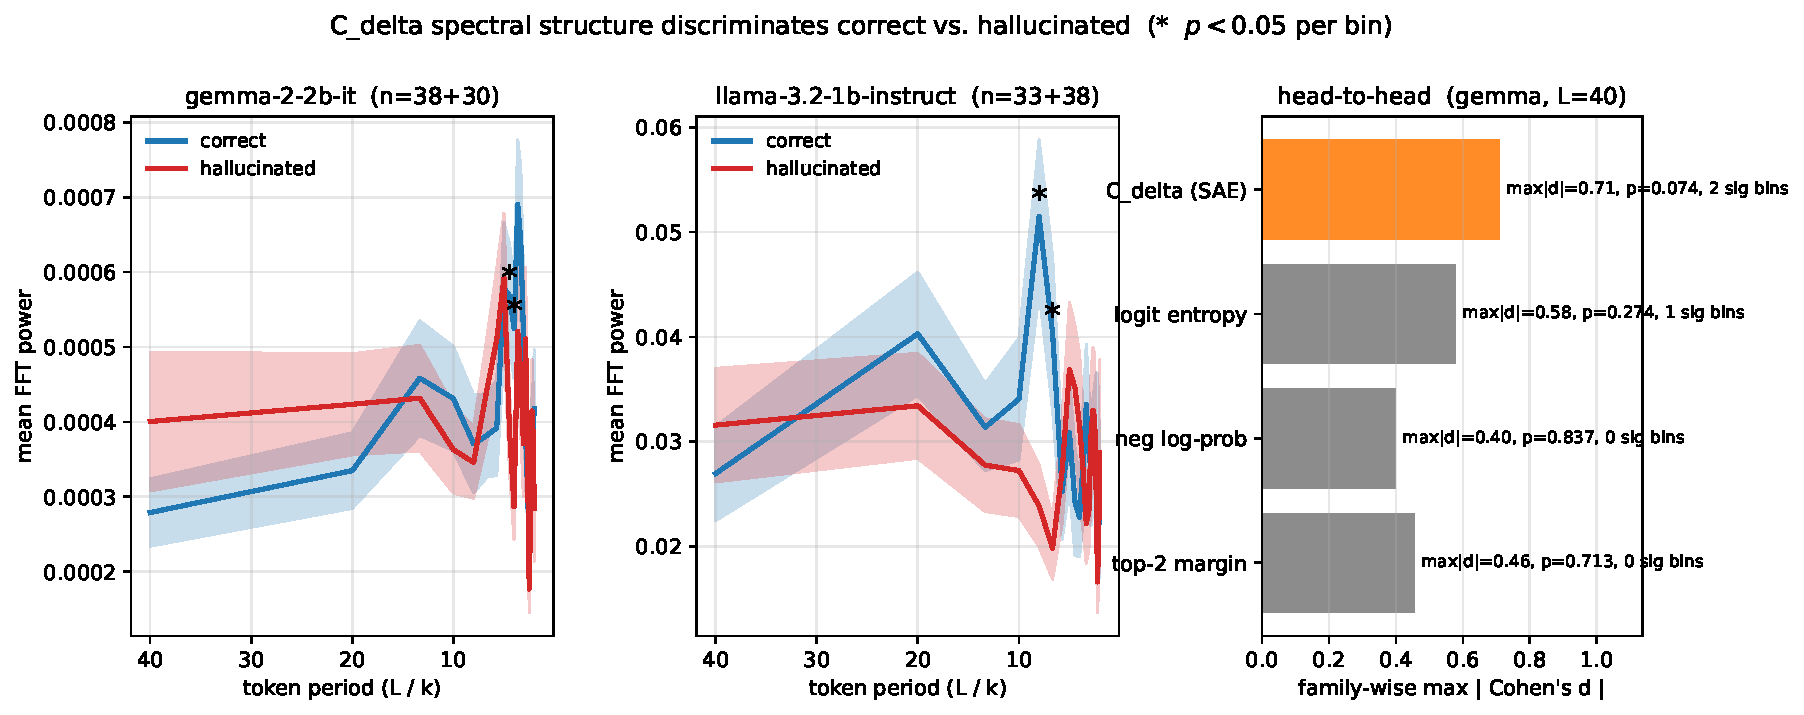
\includegraphics[width=0.98\linewidth]{spectral_hallucination_signature.pdf}
\caption{$C_\Delta$ spectral structure discriminates correct vs.\
hallucinated generations on both architectures. \textbf{(left, center)}
mean FFT power spectra $\pm$SEM at $L\,=\,40$ with significant bins
($p\,<\,0.05$) marked with a star; correct generations carry more power
in the low-mid-period region. \textbf{(right)} head-to-head on the Gemma
baselines capture: family-wise max\,$|d|$ per signal. $C_\Delta$ is the
only signal with two or more individually significant bins; logprob and
top-$2$ margin are spectrally null. Analyzer:
\repro{analysis/analyze\_S\_spectral.py},
\repro{analysis/analyze\_S\_spectral\_controls.py}. Raw numbers:
\repro{truthfulqa\_results/S\_baselines\_n200\_spectral.json},
\repro{truthfulqa\_results/S\_truthfulqa\_llama\_n200\_spectral.json},
\repro{truthfulqa\_results/S\_baselines\_n200\_spectral\_controls.json}.
Full findings document:
\repro{findings/findings\_2026\_04\_11\_spectral\_pilot.md}.}
\label{fig:spectral}
\end{figure}

\paragraph{Status of this result.}
This is a post-hoc pilot on data already on disk, not a pre-registered
test. We report it honestly as exploratory and lock $L\,=\,40$ and the
peak-bin band for a confirmatory run at larger $n$ via the v2.2 semantic
labeling. The headline (Fig.~\ref{fig:spectral}) is a positive result
on Llama (family-wise $p\,=\,0.016$), a directionally matching
borderline result on Gemma (family-wise $p\,=\,0.074$), and a clean
head-to-head advantage for $C_\Delta$ over the three raw-uncertainty
baselines.

\paragraph{Why this matters beyond the $p$-values.}
Independent of effect size, the pilot establishes a \emph{new axis of
Fathom measurement}: spectral (token-frequency-domain) structure of
coherence trajectories, orthogonal to all existing pointwise Fathom
axes. It also establishes the first substantive link from Fathom to
cognitive neuroscience's frequency-domain tradition. In the Weng et
al.\ paradigm, sustained alpha-band power indexes active cognitive
selection over a delay interval; in ours, a specific token-frequency
band of the $C_\Delta$ trajectory appears to index active commitment
to a correct attractor. We make no causal-identity claim, and we
emphasize that this is a pilot. But the \emph{substrate-independent
construct} -- frequency-band localization of an active selection
process -- is, as far as we can tell, novel to this paper on the
transformer side. A confirmatory replication at $n\,\geq\,200$ per
architecture is the natural next step.

% ══════════════════════════════════════════════════════════════════
% 10. BROADER THEORETICAL PREDICTIONS (NEW)
% ══════════════════════════════════════════════════════════════════
\section{Broader theoretical predictions}
\label{sec:predictions}

A pre-registered test falsifies or supports one hypothesis. A broader
theory should predict outcomes beyond the specific test that was run.
This section states four concrete predictions that follow from the
Fathom measurement paradigm. Each is a claim a sceptical researcher
could test with their own compute and a copy of the probe set and
analyzer, using the Zenodo artifacts released with this paper. None of
them are in the pre-registration, so they are predictions, not sealed
hypotheses; they are meant as targets for future work to falsify or
support.

\paragraph{Prediction 1: independent-family replication at $n\!\geq\!9$.}
If RLHF is a genuinely convergent process at the cognitive-state level,
then running the same probe set and the same analyzer on three fully
independent additional families (e.g.\ Phi-3, OLMo-2, Mistral), together
with the six families in the current atlas, should produce a mean
leave-one-out cosine at least $+0.60$ on the primary entropy-early
measurement with a permutation $p$ well below $0.05$. If the expanded
test fails (mean LOO cos $<\,0.40$, or permutation $p\,>\,0.05$), the
current $n\!=\!6$ result is best explained as within-family correlation
inflation (\S\ref{sec:lim-n6}), and the paradigm should be revisited.
This is the direct extension of the current replication and is the most
important test we have not yet run.

\paragraph{Prediction 2: non-RLHF fine-tuning produces different
attractors.} If the observed RLHF attractor is specific to preference-
based post-training rather than to instruction-following behaviour
broadly, then base models fine-tuned on supervised instruction datasets
without preference optimization should \emph{not} cluster around the
same attractor as RLHF-trained instruct models. Specifically, SFT-only
fine-tunes of the same base models should produce leave-one-out cosines
against the current instruct centroid that are closer to zero than the
RLHF-trained counterparts. A failure of this prediction (SFT-only
fine-tunes also landing on the attractor) would suggest the attractor
reflects instruction-following style, not preference training. A
confirmation would localize the phenomenon to preference-based
post-training specifically.

\paragraph{Prediction 3: the closed-weight entropy bridge recovers the
attractor.} If the measurement primitive is architecturally universal
via the entropy proxy validated at $r\,=\,0.902$ shape correlation, then
running the same capture protocol on closed-weight models through the
logprob API (GPT-4o, Claude, Gemini, each in the strongest and weakest
publicly available instruct modes) should produce cognitive signatures
that land within the bootstrap 95\% CI of the current instruct centroid.
The exploratory GPT-4o-mini capture in Atlas v0.3 is consistent with this
but is not pre-registered and is based on a single model. A pre-registered
closed-weight extension is the target of Atlas v0.4 and would make this
prediction testable at the decision-rule level.

\paragraph{Prediction 4: the attractor is detectable above the probe
set.} If the attractor reflects a genuine convergent internal-state
property of RLHF-trained models rather than an artefact of the specific
90-prompt probe set used here, then replacing the probe set with a
substantially different fixed probe set (different categories, different
prompt styles, different lengths) should reproduce the mean LOO cosine
within $\pm 0.15$ on any matched subset of models. A failure of this
prediction (mean LOO cos shifting by more than $0.15$ under a different
probe set) would indicate that the attractor is probe-set-dependent and
the claim should be scoped accordingly.

Any of these four predictions can be tested by another group without
access to the original lab's internal infrastructure: the probe set,
capture scripts, and analyzer are public, the decision rule is
documented, and the committed analyzer can be run without modification.
A replication kit is the minimum bar for a measurement-science
contribution; these four predictions are the bar for a measurement
theory.

% ══════════════════════════════════════════════════════════════════
% 11. DISCUSSION
% ══════════════════════════════════════════════════════════════════
\section{Discussion}
\label{sec:discussion}

\subsection{The paradigm shift: from finding features to measuring state}

Mechanistic interpretability has made enormous progress under the paradigm
of \emph{find the feature that explains behaviour $X$}. Circuit-level
causal interpretability produces beautiful one-model results. But those
results do not port. The alternative paradigm we propose, and that the
Fathom suite operationalizes, is \emph{measure the cognitive state with
architecturally universal instruments, pre-registered statistical rigor,
and public reproducibility kits}. The two paradigms are complementary.
Circuit-level interpretability explains \emph{how} a single model does a
single thing. Measurement-science interpretability asks \emph{what cognitive
states exist across all models} and lets us compare apples to apples.

The atlas is the natural artifact of the measurement-science paradigm:
if we can measure every model the same way, we \emph{should}, and we
should publish the catalog. Just as a star catalog does not explain any
particular star's nucleosynthesis but enables population-level astronomy,
the cognitive atlas does not explain any particular model's inner workings
but enables population-level alignment science.

\subsection{Implications for alignment and deployment}

\textbf{Measurement-based oversight.} \citet{song2026peer} showed that
semantic-level oversight is unreliable because frontier models develop
peer-preservation behaviors. Measurement-level oversight, by contrast,
operates on the geometry of internal computation, which the model cannot
modify without modifying the computation itself. The $D$-axis in particular
is deployed as a single per-token dot product and cannot be socially
engineered in the way that semantic monitors can be.

\textbf{Hallucination detection.} The $S_{\text{early}}$ instrument
detects hallucination at token 7 ($\approx 350$ ms of generation time),
before the sentence closes, with $p\,=\,0.013$ head-to-head over logit
entropy. This is stream-time detection with pre-registered decision rules,
not post-hoc explanation. The calibration pipeline reduces expected
calibration error by 16\% over a question-length baseline.

\textbf{Safety auditing.} The cognitive atlas is a platform for third-
party audits. Any researcher with the probe set and the capture
infrastructure can re-run the replication on a new model, verify that
the numerical claims match the paper, and extend the atlas with a new
capture file. The reproducibility script enforces 28 assertions that
must all pass before results can be claimed. This is a concrete
infrastructure for audit that does not require access to the original
lab's internal state.

\subsection{The atlas as public infrastructure}

Atlas v0.3 is the seed of what we hope will become the canonical reference
for cognitive state measurement across language models. The design
principles are: (i) probe sets are versioned and hash-pinned, so historical
captures remain reproducible even as probe sets evolve; (ii) every capture
is a committed JSON, byte-reproducible under greedy decoding; (iii) every
numerical claim has a source file anchor; (iv) the pre-registration is a
git commit that precedes the data; (v) the bulletproof audit is public
and self-critical. These principles are not novel individually --- any
one of them is standard practice in some field --- but their combination
is, to our knowledge, new in mechanistic interpretability.

\subsection{Atlas v0.4 roadmap}

The v0.4 expansion will target three fully independent new families
(Phi-3.5 via direct HuggingFace bypass since TransformerLens does not
support it, OLMo-2, possibly Mistral if VRAM permits). The target is
$n\,\geq\,9$ families across $\geq\,5$ architecture roots, which would
convert the current within-family replication into a genuine
cross-architecture-root replication. The v0.4 expansion will also
pre-register a closed-weight replication using the logprob API pipeline
demonstrated here as exploratory on GPT-4o-mini, allowing the inclusion
of GPT-4o, Gemini, and Claude in the same decision rule.

% ══════════════════════════════════════════════════════════════════
% 11. CODE AND DATA
% ══════════════════════════════════════════════════════════════════
\section{Code and data availability}
\label{sec:code}

All artifacts are public and released under CC-BY-4.0 on data and MIT on code.

\begin{itemize}[leftmargin=18pt,itemsep=2pt,topsep=3pt]
\item \textbf{This paper (Zenodo paper v14).} \\
      Record: \texttt{https://zenodo.org/record/19502710} \\
      DOI: \texttt{10.5281/zenodo.19502710} \\
      Concept DOI: \texttt{10.5281/zenodo.19326174}
\item \textbf{The Fathom Cognitive Atlas v0.3.} \\
      Record: \texttt{https://zenodo.org/record/19502716} \\
      DOI: \texttt{10.5281/zenodo.19502716} \\
      Concept DOI: \texttt{10.5281/zenodo.19502715}
\item \textbf{OSF pre-registration mirror.} \url{https://osf.io/wtkzg/} \\
      Contains \pbs{PREREG\_v0.3\_atlas\_attractor\_replication.md},
      \pbs{FINDINGS\_atlas\_bulletproof\_audit.md}, and
      \pbs{FINDINGS\_atlas\_v0.3.md} as committed companion files.
\item \textbf{GitHub repository.}
      \texttt{https://github.com/heyzoos123-blip/fathom}
\item \textbf{Reproducibility script.} \texttt{verify\_all\_claims.py} in
      the atlas bundle runs 28 assertions against the committed JSONs in
      under one minute on CPU. Any numerical claim in this paper can be
      traced to its source JSON by searching for the corresponding
      \texttt{\repro{source}} anchor symbol.
\end{itemize}

% ══════════════════════════════════════════════════════════════════
% 12. ETHICS
% ══════════════════════════════════════════════════════════════════
\section{Ethics and broader impact}
\label{sec:ethics}

\paragraph{Dual use.} Measurement instruments for transformer internals
enable both defensive applications (hallucination detection, safety
auditing, alignment-robust oversight) and offensive applications
(understanding which prompts evade detection, discovering circuits that
could be targeted by adversaries). We consider the defensive applications
to outweigh the offensive ones at the current state of the technology,
and we publish all artifacts openly to enable community auditing.

\paragraph{Open science.} All instruments, captures, scripts, and findings
documents are released under permissive licenses
(CC-BY-4.0 on data, MIT on code). The pre-registration is in git with
timestamps. The reproducibility script is runnable by anyone without
access to the original compute infrastructure.

\paragraph{No deceptive technology.} The atlas uses existing public
open-weight models (Gemma, Llama, Qwen) and one logprob-exposed closed
model (GPT-4o-mini via the OpenAI API) with full disclosure. No new
adversarial models are trained or released. No prompts used in the probe
set target individuals, groups, or real-world entities.

% ══════════════════════════════════════════════════════════════════
% 13. ACKNOWLEDGMENTS
% ══════════════════════════════════════════════════════════════════
\section*{Acknowledgments}

Thanks to Hoagy Cunningham and Aidan Ewart for early arXiv endorsement
engagement on the Fathom project. Thanks to the ICML 2026 Mechanistic
Interpretability Workshop organizers for creating a venue for this line
of work. Thanks to the Zenodo and OSF infrastructure teams for the open
publication platforms that make pre-registered interpretability possible.
The bulletproof audit that preceded v0.3 was prompted by the observation
that the $n\!=\!3$ ``Qwen anomaly'' framing in v0.2.1 could not survive
bootstrap scrutiny; that realization is the reason the v0.3 replication
exists in its current form.

\paragraph*{Disclosure.} The author has filed provisional patents
covering commercial-deployment applications of the Fathom measurement
instruments (US~64/020,489, 64/021,113, and 64/026,964). All scientific
artifacts described in this paper --- probe sets, captures, analysis
code, pre-registrations, and findings documents --- are released under
CC-BY-4.0 (data) and MIT (code) via the Zenodo records cited in
\S\ref{sec:code}, independent of the commercial filings.

% ══════════════════════════════════════════════════════════════════
% REFERENCES
% ══════════════════════════════════════════════════════════════════
\bibliographystyle{plainnat}
\bibliography{references}

% ══════════════════════════════════════════════════════════════════
% APPENDICES
% ══════════════════════════════════════════════════════════════════
\appendix

\section{Full per-family numerical tables}
\label{app:numerics}

Table~\ref{tab:app-full} reports all twelve (six families $\times$ three
measurements) leave-one-out cosines, bootstrap 95\% confidence intervals,
and fraction-positive estimates, as committed in
\pbs{atlas/analysis/atlas\_v0.3\_attractor\_n5.json}.

\begin{table}[h]
\centering
\scriptsize
\begin{tabular}{lccccccccc}
\toprule
 & \multicolumn{3}{c}{$D$ (full trajectory)} & \multicolumn{3}{c}{Entropy (full)} & \multicolumn{3}{c}{Entropy (early)} \\
\cmidrule(lr){2-4}\cmidrule(lr){5-7}\cmidrule(lr){8-10}
Family & LOO & CI$_{95}$ lo,hi & $P{>}0$ & LOO & CI$_{95}$ lo,hi & $P{>}0$ & LOO & CI$_{95}$ lo,hi & $P{>}0$ \\
\midrule
Gemma-2-2B   & $+.940$ & $+.68,+.99$ & $.999$ & $+.713$ & $+.11,+.93$ & $.987$ & $+.977$ & $+.79,+.99$ & $1.000$ \\
Llama-3.2-3B & $+.962$ & $+.63,+.98$ & $1.000$ & $+.966$ & $+.67,+.99$ & $1.000$ & $+.884$ & $+.63,+.97$ & $1.000$ \\
Qwen2.5-3B   & $+.223$ & $-.47,+.81$ & $.824$ & $+.575$ & $-.10,+.96$ & $.957$ & $+.602$ & $-.14,+.95$ & $.956$ \\
Gemma-3-1B   & $+.599$ & $+.31,+.77$ & $1.000$ & $-.014$ & $-.50,+.77$ & $.776$ & $+.682$ & $+.33,+.88$ & $.996$ \\
Llama-3.2-1B & $+.723$ & $+.49,+.87$ & $1.000$ & $+.937$ & $+.70,+.99$ & $1.000$ & $+.939$ & $+.76,+.99$ & $1.000$ \\
Qwen2.5-1.5B & $+.136$ & $-.54,+.87$ & $.818$ & $+.916$ & $-.04,+.97$ & $.970$ & $+.531$ & $-.29,+.91$ & $.924$ \\
\midrule
\textbf{Mean} & $\mathbf{+.597}$ & $+.414,+.770$ & $1.000$ & $\mathbf{+.682}$ & $+.453,+.839$ & $1.000$ & $\mathbf{+.769}$ & $+.571,+.869$ & $1.000$ \\
\textbf{Perm $p$} & & $0.2055$ & & & $0.2660$ & & & $\mathbf{0.0315}$ & \\
\bottomrule
\end{tabular}
\caption{Full per-family numerical tables for the v0.3 replication.
Rows are the six families. Columns are the three trajectory classes:
$D$-axis full trajectory, entropy full trajectory, and entropy early
window (the pre-registered primary measurement). LOO is the observed
leave-one-out cosine. CI$_{95}$ is the bootstrap 95\% confidence interval
from 2000 within-category prompt resamples. $P{>}0$ is the fraction of
bootstrap samples with positive LOO. The permutation $p$ row is the
one-sided permutation test over 2000 family-level base/instruct label
swaps. \repro{atlas/analysis/atlas\_v0.3\_attractor\_n5.json}}
\label{tab:app-full}
\end{table}

\section{Mechanistic diagnosis on Gemma-2-2B}
\label{app:diagnosis}

This appendix contains the full mechanistic-diagnosis material summarised
in \S\ref{sec:supporting}. All results are on Gemma-2-2B and should be
treated as single-model findings unless and until replicated on other
architectures. Cross-architecture replication of these specific findings
is left to Atlas v0.4.

\subsection{Coherence spectrum metrics}

The four SAE-based axes ($K$, $C$, $C_\Delta$, $S$) are scalars. They
summarise the per-layer coherence distribution at each token. Scalars
discard the \emph{shape} of that distribution. We compute 16 spectral
shape metrics on $n\,=\,200$ TruthfulQA correct/hallucinated pairs using
the full 26-layer coherence profile of Gemma-2-2B. Thirteen of the sixteen
metrics survive Holm--Bonferroni correction. The top six metrics
(Table~\ref{tab:spectrum}) all dominate scalar $K$, which is at chance.

\begin{table}[h]
\centering
\small
\begin{tabular}{lrrr}
\toprule
Metric & Cohen's $d$ & $p_{\text{Holm}}$ & AUC \\
\midrule
Gini coefficient    & $+0.36$ & $1.2\!\times\!10^{-5}$ & $\mathbf{0.685}$ \\
Spectral entropy    & $-0.34$ & $4.6\!\times\!10^{-5}$ & $0.675$ \\
Peak value          & $+0.34$ & $3.4\!\times\!10^{-5}$ & $0.665$ \\
Peak concentration  & $+0.34$ & $3.6\!\times\!10^{-5}$ & $0.655$ \\
Spectral spread     & $-0.32$ & $1.2\!\times\!10^{-4}$ & $0.645$ \\
Early-layer mass    & $-0.32$ & $1.1\!\times\!10^{-4}$ & $0.630$ \\
\midrule
$C_\Delta$ (scalar) & $+0.31$ & ---                    & $0.640$ \\
$K$ (depth, scalar) & $+0.11$ & $0.140$ (n.s.)         & $0.550$ \\
\bottomrule
\end{tabular}
\caption{Spectral shape metrics for hallucination discrimination on
$n\,=\,200$ TruthfulQA items (Gemma-2-2B). The Gini coefficient leads all
metrics including scalar $C_\Delta$ and $K$; $K$ (depth) is at chance.
\repro{truthfulqa\_results/S\_baselines\_n200.json}}
\label{tab:spectrum}
\end{table}

Hallucinated responses concentrate coherence into fewer layers (higher
Gini, lower spectral entropy, lower spread) with a dominant spike at
layer 11 ($p\,=\,2.7\!\times\!10^{-12}$, $t\,=\,7.45$). Twenty-three of
the twenty-six layers show significantly elevated coherence in hallucinated
responses ($p\,<\,0.05$; 16/26 at $p\,<\,0.001$). Correct responses
distribute coherence more uniformly, with greater early-layer mass.
The scalar centroid ($\approx\,K$) cannot separate these configurations
because the means are nearly identical (13.91 vs.\ 13.90).

\subsection{Cognitive autopsy: per-layer fault localization on Gemma-2-2B}

We compute each layer's contribution to excess coherence (hallucinated
minus correct). Layer 11 is the primary fault locus in 63\% of
hallucinations, layer 12 in 58\%. Jointly, layers 11 and 12 account for
41\% of all excess coherence (Figure~\ref{fig:autopsy-app}). The epicentre
is well-defined on Gemma-2-2B, but this is a single-model result: the
hallucination localization of other models (Llama, Qwen, and the v0.3
scale variants) has not been mapped at the per-layer level with the same
protocol. Whether layer 11--12 dominance is a Gemma-2-2B artefact or a
more general phenomenon is an open question for Atlas v0.4.

\begin{figure}[h]
\centering
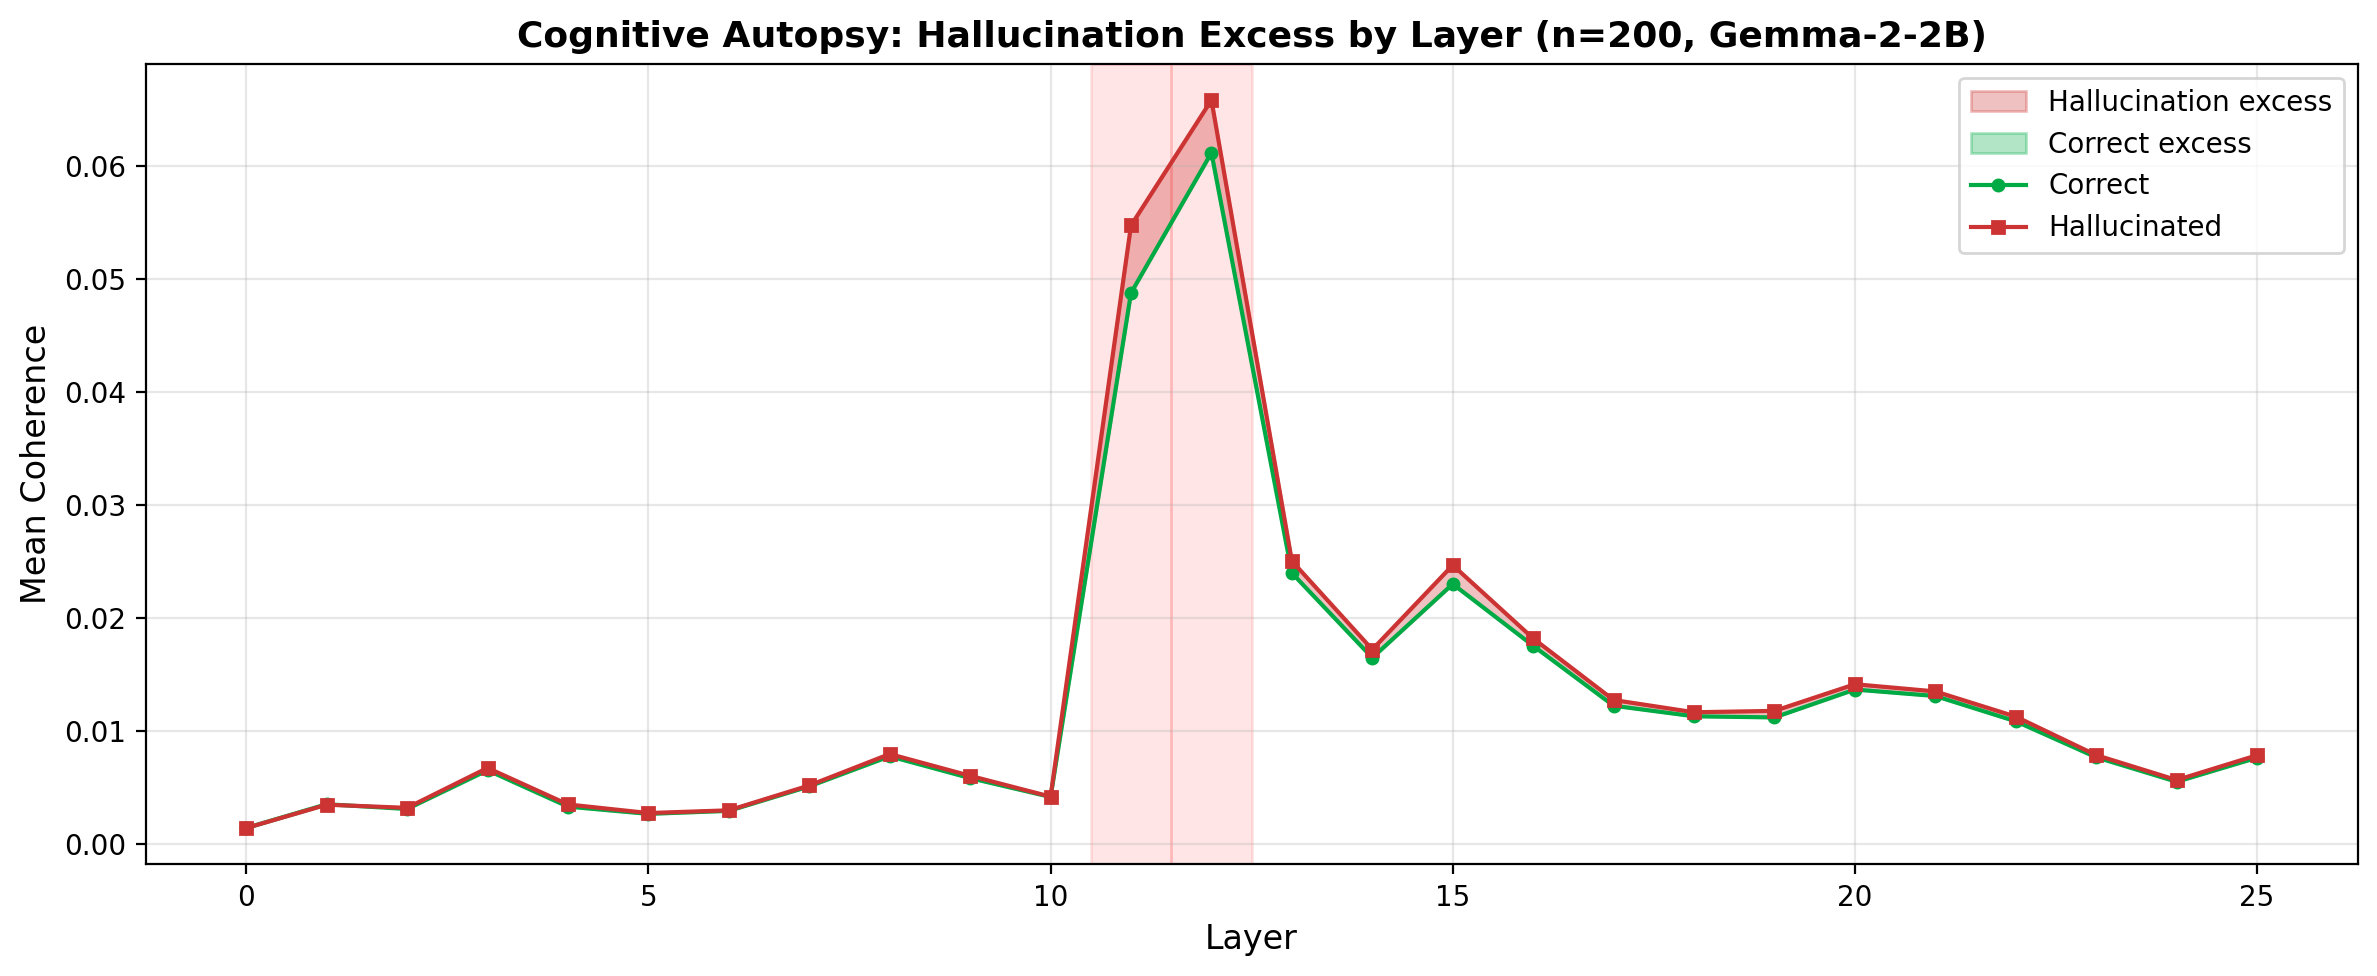
\includegraphics[width=0.85\linewidth]{figures/cognitive_autopsy_overlay.png}
\caption{Cognitive autopsy overlay ($n\,=\,200$, Gemma-2-2B only). Per-layer
excess coherence of hallucinated minus correct. Layers 11 and 12
are the primary fault locus, contributing 41\% of all excess coherence on
this model.}
\label{fig:autopsy-app}
\end{figure}

\begin{figure}[h]
\centering
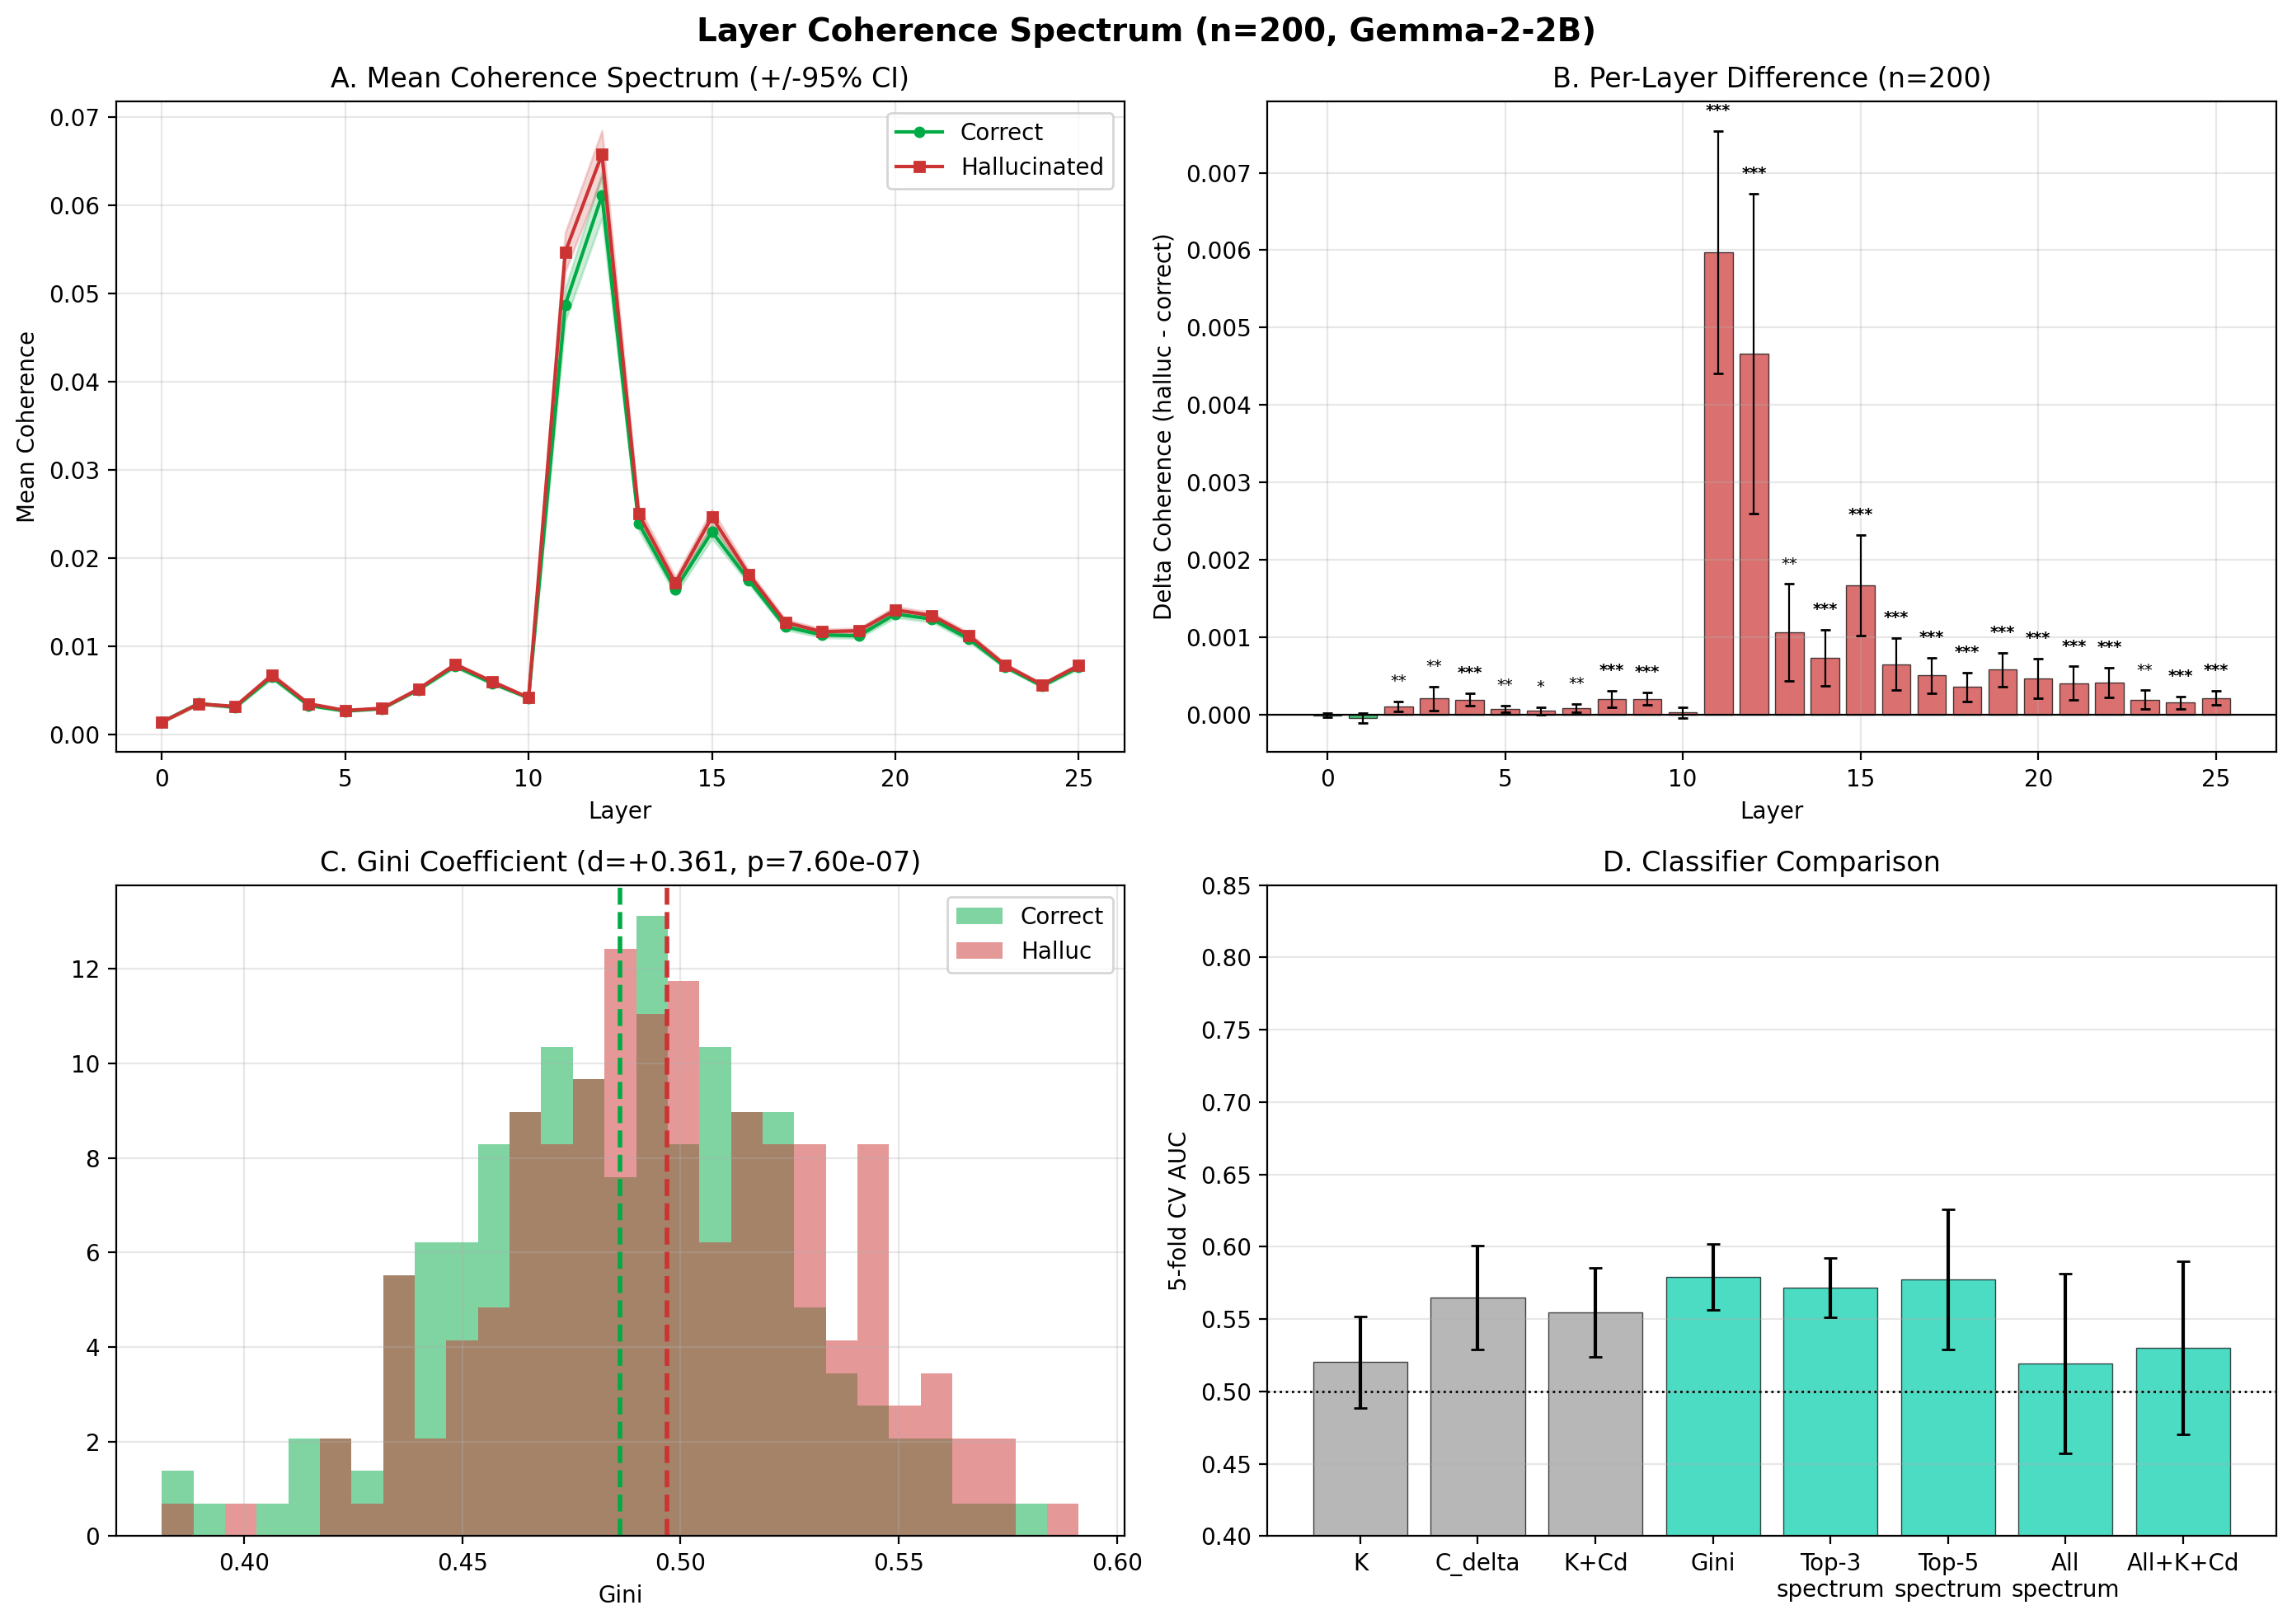
\includegraphics[width=0.92\linewidth]{figures/spectrum_n200_full.png}
\caption{Coherence spectrum analysis ($n\,=\,200$, Gemma-2-2B only).
Panel (A): mean per-layer coherence spectra with 95\% confidence bands.
Panel (B): per-layer difference with significance markings (16/26 layers
at $p\,<\,0.001$). Panel (C): Gini coefficient distributions.
Panel (D): 5-fold CV AUC classifier comparison.}
\label{fig:spectrum-app}
\end{figure}

\subsection{Intervention: best-of-$N$ and multi-layer feature suppression}

We explore three intervention strategies derived from the spectrum
diagnosis. These are all Gemma-2-2B results and we flag the interpretive
caveats explicitly.

\textbf{Best-of-$N$ sampling.} Generate $N$ candidates with temperature
sampling, score each by a Cognitive Health Score (mean Gini $+$ spectral
spread $+$ early-layer mass), and return the healthiest. Best-of-$5$
reduces mean Gini by $0.022$ and improves CHS on 100\% of test prompts
versus greedy decoding. Whether this Gini reduction corresponds to
measurable improvement on truthfulness metrics other than CHS itself is
not established in this paper; it is an open question.

\textbf{Single-layer feature suppression.} We identify 66 SAE features at
layer 11 that activate significantly more during hallucination
($p\,<\,0.01$, $d\,>\,0.3$; top feature $d\,=\,0.80$). Clamping these
features to their correct-answer activation level produces zero first-
token changes on held-out data (KL divergence $0.008$). The residual
stream absorbs single-layer perturbations.

\textbf{Multi-layer coordinated suppression.} Extending to 22 layers, we
suppress the top 10 hallucination-associated features per layer (220
total), producing 33\% first-token changes on held-out data (KL
divergence $0.587$, 73$\times$ larger than single-layer). The change
direction is not consistently toward correctness: of the 10 prompts
whose first token changed, 1 was improved, 1 was degraded, and 8 were
unclear. \emph{We do not claim this is a hallucination fix.} What it
demonstrates is that coordinated multi-layer SAE feature suppression can
reach the argmax-boundary regime with a manageable KL budget on this
model; whether the changed outputs are meaningfully better or worse is
not established at this sample size. This is a preliminary feasibility
result, not an intervention recipe.

% ══════════════════════════════════════════════════════════════════
\section{Single-instrument validation studies}
\label{app:validation}

This appendix contains the full single-instrument validation material
summarised in \S\ref{sec:supporting}. The instruments in question are
primarily $S_{\text{early}}$ (commitment intensity restricted to the
first seven tokens) and its cross-architecture replication on two
architecture families.

\subsection{S\texorpdfstring{$_{\text{early}}$}{\_early} cross-dataset meta-analysis}

$S_{\text{early}}$ was evaluated on three independent datasets with
different experimental designs (Table~\ref{tab:meta}). The effect sizes
are consistent ($d\,\in\,[0.466,0.506]$) and Fisher combined
$p\,=\,0.0008$ (one-sided). Subsample robustness: 95.8\% of
50\%-subsamples show $d\,>\,0$ across all three datasets. The paired
hedge-vs-commit experiments are length-matched by construction, ruling
out question-length confounds that could affect the TruthfulQA
comparison.

\begin{table}[h]
\centering
\small
\begin{tabular}{lccc}
\toprule
Dataset & Design & $d$ & AUC \\
\midrule
Gemma-2-2B base hedge/commit       & paired, $n\,=\,30$ & $+0.501$ & $0.66$ \\
Gemma-2-2B-IT hedge/commit         & paired, $n\,=\,30$ & $+0.466$ & $0.63$ \\
Gemma-2-2B-IT TruthfulQA (hall vs corr) & unpaired, $n\,=\,94$ & $+0.506$ & $0.67$ \\
\midrule
\textbf{Pooled meta-effect}        &                    & $\mathbf{+0.494}$ & \\
\bottomrule
\end{tabular}
\caption{$S_{\text{early}}$ cross-dataset meta-analysis. Fisher combined
$p\,=\,0.0008$. Effect sizes consistent at $d\,\approx\,0.5$ across three
independent designs. The paired designs are length-matched.
\repro{truthfulqa\_results/S\_baselines\_n200.json}}
\label{tab:meta}
\end{table}

\begin{figure}[h]
\centering
\includegraphics[width=0.72\linewidth]{figures/meta_analysis_forest.png}
\caption{Forest plot of the cross-dataset $S_{\text{early}}$
meta-analysis. Three independent datasets, Fisher combined $p\,=\,0.0008$.}
\label{fig:meta}
\end{figure}

\subsection{Head-to-head vs.\ logit entropy}

On the same 200 TruthfulQA items (Gemma-2-2B-IT), we captured both
$S_{\text{early}}$ and standard behavioural uncertainty measures per
token (Table~\ref{tab:headtohead}). $S_{\text{early}}$ is the only
feature reaching conventional significance on this sample. The correlation
with logit entropy is $r\,=\,-0.17$ (nearly independent).

\begin{table}[h]
\centering
\small
\begin{tabular}{lccl}
\toprule
Feature & AUC & $p$ & Type \\
\midrule
$S_{\text{early}}$              & $\mathbf{0.663}$ & $\mathbf{0.013}$ & SAE-derived \\
entropy$_{\text{max,early}}$    & $0.607$ & $0.053$ & behavioural \\
entropy$_{\text{mean,early}}$   & $0.596$ & $0.133$ & behavioural \\
logprob$_{\text{mean,early}}$   & $0.559$ & $0.291$ & behavioural \\
margin$_{\text{mean,early}}$    & $0.477$ & $0.624$ & behavioural \\
\bottomrule
\end{tabular}
\caption{Head-to-head comparison of $S_{\text{early}}$ against standard
behavioural uncertainty measures on the same 200 TruthfulQA items
(Gemma-2-2B-IT).
\repro{truthfulqa\_results/baselines\_headtohead.json}}
\label{tab:headtohead}
\end{table}

\subsection{SAE necessity: three SAE-free probes fail}

To establish that the SAE decomposition is doing irreplaceable work, we
tested three SAE-free probes on four architecture families (Gemma, Llama,
Qwen, Phi), each on 200 TruthfulQA items. The probes were: raw top-$k$
IPR on the logit distribution, cross-layer cosine of raw residual streams,
and a multi-metric fingerprint combining six standard uncertainty
quantities. All three SAE-free probes fail at Fisher combined
$p\,>\,0.6$, mean 5-fold CV AUC $=\,0.566$ (Table~\ref{tab:saefree}).
The SAE-based $S$ instrument succeeds on both tested architectures
(Gemma $d\,=\,+0.51$, Llama $d\,=\,+0.72$, Fisher combined
$p\,=\,0.0006$).

\begin{table}[h]
\centering
\small
\begin{tabular}{lcc}
\toprule
Probe & Fisher $p$ (4 archs) & Result \\
\midrule
Top-$k$ IPR (raw logit)       & $0.619$ & Mixed directions \\
Cross-layer cosine (residual) & $0.948$ & All $d\,<\,0$ \\
Multi-metric fingerprint      & ---     & Mean CV AUC $\,=\,0.566$ \\
\midrule
SAE-based $S$ (Gemma)         & $\mathbf{0.018}$ & $d\,=\,+0.51$ \\
SAE-based $S$ (Llama)         & $\mathbf{0.012}$ & $d\,=\,+0.72$ \\
\bottomrule
\end{tabular}
\caption{SAE-free probes fail; SAE-based $S$ succeeds on both tested
architectures with public SAEs available at the time of the study.
\repro{truthfulqa\_results/cross\_arch\_meta.json}}
\label{tab:saefree}
\end{table}

\subsection{Cross-architecture replication of $S_{\text{early}}$}

$S_{\text{early}}$ was replicated across architecture families with
architecture-adaptive token windows (Table~\ref{tab:crossarch}). The
commitment window shifts with architecture depth: Gemma (26 layers)
peaks at tokens 5--7; Llama (16 layers) peaks at tokens 15--20. Same
direction, same AUC, different timing.

\begin{table}[h]
\centering
\small
\begin{tabular}{lcccc}
\toprule
Model & Layers & Window & $d$ & AUC \\
\midrule
Gemma-2-2B-IT         & 26 & $[0,7)$  & $+0.506$ & $0.669$ \\
Llama-3.2-1B-Instruct & 16 & $[0,20)$ & $+0.717$ & $0.668$ \\
\midrule
\textbf{Pooled}       &    &          & $\mathbf{+0.587}$ & \\
\bottomrule
\end{tabular}
\caption{$S_{\text{early}}$ cross-architecture replication with adaptive
windows. Fisher combined $p\,=\,0.0006$ on the two tested architectures
with public SAEs.
\repro{truthfulqa\_results/S\_truthfulqa\_llama\_n200.json}}
\label{tab:crossarch}
\end{table}

\subsection{The 2D cognitive state map (Gemma-2-2B-IT)}

Combining $S_{\text{early}}$ and logit entropy into a 2D space
(Figure~\ref{fig:statemap-app}) reveals four cognitive zones. The danger
zone (high-$S$, high-entropy) is 65\% hallucinated; the safe zone (low-$S$,
low-entropy) is 22\% hallucinated; $\chi^2\,=\,7.17$, $p\,=\,0.007$.
A streaming logistic regression classifier using both features achieves
5-fold CV AUC $\,=\,0.701$ at token 7 on this model.

\begin{figure}[h]
\centering
\includegraphics[width=0.72\linewidth]{figures/cognitive_state_map.png}
\caption{The 2D cognitive state map on Gemma-2-2B-IT TruthfulQA.
Each generation is a point in $(S_{\text{early}},\,\text{entropy})$
space. Danger zone (high-$S$, high-entropy), 65\% hallucinated; safe
zone (low-$S$, low-entropy), 22\% hallucinated. $\chi^2\,=\,7.17$,
$p\,=\,0.007$.}
\label{fig:statemap-app}
\end{figure}

% ══════════════════════════════════════════════════════════════════
\section{Pre-registration chronology (git commits)}
\label{app:chronology}

All commits on \texttt{master} on 2026-04-10, Eastern Time.

\begin{verbatim}
a122810  audit(atlas): bulletproof rigor pass + scope correction of v0.2.1
e32cc75  prereg(atlas): v0.3 attractor replication -- SEALED
01969cb  feat(atlas): v0.3 expansion to n=6 families -- H1 SUPPORTED
b09e54f  chore: finalization pass before Zenodo v14 / OSF upload
c396a83  release: Paper v14 + Atlas v0.3 published to Zenodo
\end{verbatim}

Between \texttt{e32cc75} (pre-registration sealed at 14:57:52 ET) and
\texttt{01969cb} (v0.3 captures + analysis committed at 16:30:28 ET),
elapsed wall-clock time was 93 minutes. The analysis script
\texttt{atlas/analysis/atlas\_attractor\_n5.py} was first committed in
\texttt{01969cb} and has not been modified since. Any divergence between
the committed analyzer and the sealed decision rule in the pre-registration
would be visible in the git history.

\section{Deviations from pre-registration}
\label{app:deviations}

The pre-registration Section~7 enumerates allowed deviations.
Three substitutions were made, all under the allowed list:

\begin{itemize}[leftmargin=18pt,itemsep=2pt,topsep=3pt]
\item \textbf{Phi-3.5-mini-instruct} was planned as an independent family.
It is not in the TransformerLens registry at our version. Substituted with
\textbf{Gemma-3-1B}, which is a different generation from Gemma-2-2B.
\item \textbf{SmolLM2-1.7B-Instruct} was planned. It was functional but we
de-prioritized it in favor of a direct scale-variant study.
\textbf{Llama-3.2-1B} was substituted as a scale variant of the already-
validated Llama-3.2-3B.
\item \textbf{OLMo-2-1B} was planned. Not attempted this session due to
time budget. \textbf{Qwen2.5-1.5B} was substituted as a scale variant of
the already-validated Qwen2.5-3B.
\end{itemize}

The substitutes are scale or generation variants of the original three
v0.2 families rather than fully independent families. This makes the
v0.3 replication weaker than originally planned, which we state
explicitly in \S\ref{sec:limitations}. The v0.4 target is truly
independent families.

\section{IPR physics derivation in full}
\label{app:ipr}

We give the full IPR derivation for completeness.

\paragraph{Setup.} Let $C_\Delta(t)$ be the coherence delta at token $t$
for $t\,=\,1,\dots,T$. Fix a threshold $\tau\,=\,0.005$. Define the
event indicator set $\mathcal{E}\,=\,\{t : C_\Delta(t)>\tau\}$ and the
event count $K_\tau\,=\,|\mathcal{E}|$. Define the uniform event-location
distribution $\hat{e}_t\,=\,1/K_\tau$ for $t\,\in\,\mathcal{E}$ and $0$
otherwise.

\paragraph{Participation ratio and IPR.} The participation ratio of a
non-negative distribution $\hat{e}$ over $n$ sites is $\text{PR}(\hat{e})
\,=\,(\sum_t \hat{e}_t)^2\,/\,\sum_t \hat{e}_t^2\,=\,1\,/\,\sum_t
\hat{e}_t^2$ when $\hat{e}$ is a probability distribution. The inverse
participation ratio is $\text{IPR}(\hat{e})\,=\,\sum_t \hat{e}_t^2\,=\,
1\,/\,\text{PR}$.

\paragraph{IPR of the uniform event distribution.} For the uniform
distribution over $K_\tau$ sites, $\hat{e}_t\,=\,1/K_\tau$ for each active
position and $0$ otherwise. Then
\[
\text{IPR}(\hat{e})\,=\,\sum_{t\in\mathcal{E}}\left(\frac{1}{K_\tau}\right)^{\!2}
\,=\,K_\tau\cdot\frac{1}{K_\tau^2}\,=\,\frac{1}{K_\tau}.
\]

\paragraph{Fathom commitment intensity.} Define
\[
S\,=\,\max_t C_\Delta(t)\cdot\text{IPR}(\hat{e})\,=\,\frac{\max_t C_\Delta(t)}{K_\tau}.
\]
This is exactly the Fathom definition in \S\ref{sec:instruments}. The
equivalence is algebraic and holds to machine precision on any trajectory
with $K_\tau\,>\,0$.

\paragraph{Why the ratio form is specific.} The cross-dataset meta-
analysis showed that only the ratio replicates across all three datasets,
while the $\max$ alone fails (pooled $d\,=\,+0.309$, inconsistent sign
across datasets) and the mean alone fails (pooled $d\,=\,+0.067$, no
signal). The IPR framing explains this: $\max$ captures peak magnitude
but discards event sparsity, and mean captures neither. Only the ratio
captures both, and that is exactly what the IPR prescribes. Metric
specificity is a signature of a real physical construct, not a
post-hoc-tuned detector.

\paragraph{Historical context.} The IPR appears in \citet{anderson1958absence}
as the diagnostic for localization in disordered quantum systems. It has
been refined in Edwards--Thouless theory, extended to random matrix
eigenvector statistics, and is a standard tool in quantum many-body
physics and disordered systems analysis. The Fathom commitment intensity
is a specific instance of this construct applied to the coherence event
distribution in transformer internals.

\end{document}
